\chapter{On the production of entangled beams from a metastable Helium BEC}
\label{Peaks}
\graphicspath{{Figures/Peaks/}{Figures/Common/}}

The results presented in this chapter have been published in \citet{Dall:2009}. All of the theoretical work in this paper except as noted in this chapter was my own work.

\section{Introduction}
Sources of matter waves gained a dramatic improvement with the achievement of Bose-Einstein condensation (BEC) in dilute gases and the development of the atom laser \citep{Anderson:1995vn,Mewes:1997}. Like optical lasers before them, atom lasers can produce Heisenberg-limited beam profiles \citep{Busch:2002zr,Riou:2006uq} and promise high spectral density through their dramatically lower linewidth \citep{Wiseman:1997ba}. Another exciting possibility resulting from having such a coherent source of atoms is the generation of nonclassical matter waves through entangled beams. Such entangled beams are useful for tests of quantum mechanics and are required to perform Heisenberg-limited interferometry \citep{Dowling:1998,Reid:1988}. In this chapter, we show that the asymmetric scattering lengths between internal states of metastable helium (He*) cause well-defined peaks in the output of an atom laser. These peaks are due to a phase-matched four-wave mixing (FWM) process and are experimentally demonstrated.

A nonlinear process is required to produce entanglement, and one of the advantages of atomic systems over optical systems is that there are strong inherent nonlinearities due to atomic interactions, although these interactions can also lead to complications. These nonlinearities allow certain analogues of nonlinear optical experiments such as four-wave mixing (FWM) and Kerr squeezing to be performed directly in the atomic sample \citep{WallsMilburn}. All of these produce entanglement in optical systems. Four-wave mixing in a trapped BEC has been demonstrated experimentally in configurations where three distinct momentum states generated a fourth \citep{Deng:1999qy} and where two momentum states generated a pair of correlated atomic beams \citep{Vogels:2002}. These experiments demonstrated that the output phase was coherent, but the correlation properties were not measured. More recently the pair correlations in a spontaneous scattering of two colliding condensates were measured using the single-atom detectors available for He* atoms \citep{Perrin:2007}.

Using these existing sources of entangled pairs of atoms for interferometric experiments will be complicated by the high densities of the sources, where the nonlinearities that generated the correlations ultimately degrade the long-term coherence of the sample. While recent experiments have increased the coherence of atom interferometers by several orders of magnitude by reducing the nonlinearities with a Feschbach resonance \citep{Fattori:2008,Gustavsson:2008}, this precludes the production of entangled pairs. In our scheme the nonlinear interactions are used to drive FWM in the magnetically untrapped condensate, but the resulting untrapped beams that propagate in free space are dilute, potentially avoiding the decoherence problem. We show that pairs of beams can be produced simply by the process of radio-frequency (rf) outcoupling from a He* BEC, without the need for Feschbach resonances, optical traps, or scattering pulses. Unlike previous methods, which required pairs of atoms travelling at high kinetic energies as a source, this process involves scattering between atoms initially in the same zero-momentum state to create states with nonzero momentum. Semiclassical and field-theoretic simulations of the experiment show that the beams are generated by the same FWM process that generated entangled atom pairs in the earlier experiments.

\section{The metastable Helium `Peaks' experiment}
\label{Peaks:ExperimentalSetup}

The experimental setup for creating He* BEC has been reported elsewhere \citep{Dall:2007a}, and discussed earlier in this thesis (see \sectionref{He*Experiment}\footnote{FIXME: Correct this reference when this section is written}). The experiment discussed in this section was performed by \emph{Robert Dall}, \emph{Lesa Byron} and \emph{Andrew Truscott} at the Research School of Physics and Engineering, ANU.

Starting from an almost pure BEC containing up to $5\times 10^6$ atoms an atom laser beam was created by using rf photons to spin flip the BEC atoms from the $m=1$ magnetically trapped state to the $m=0$ untrapped state.

After outcoupling, atoms in the atom laser beam fell under gravity for a distance of $\unit[4]{cm}$ until they hit a double stacked multichannel plate (MCP). The phosphor screen was imaged with a charge-coupled-device (CCD) camera with a resolution of approximately $\unit[150]{\micro m}$ at the MCP. To remove any nonuniformities caused by spatial variations in the gain of the MCP, all images were divided by a flat-field image produced by dropping atoms from a MOT onto the detector. Since the MOT temperature is of order $\sim\unit[1]{mK}$, the spatial profile of the MOT uniformly illuminates the MCP. Although $m=-1$ atoms are produced by the outcoupling, especially for high rf powers, they are in general accelerated away from the detector by the magnetic trap field. Those that are accelerated towards the detector do not show up in the images since they arrive much earlier than the CCD trigger time.

\figureref{Peaks:ExperimentalResults} shows the dramatic change in the atom laser spatial profile when the condensate undergoes the resonant FWM process. In the case of low outcoupling Rabi frequencies (upper row), the FWM process does not occur and we see the usual double-peaked He*-atom laser profile \citep{Dall:2007} (see also \sectionref{TransverseProfile:Helium}\footnote{FIXME: Correct this reference when this section is written}). When the Rabi frequencies are high enough to initiate the FWM process (lower row), the atoms in the atom laser beam are scattered to form a halo around the main atom laser beam. Due to conservation of energy, the outer diameter of this halo corresponds to a maximum kinetic energy given by the chemical potential. As well as the ring structure, four peaks are observed on the outskirts of the profile.
% Each peak contains 11\%--14\% of the total outcoupled atoms, in agreement with the value of 11\% obtained from the simulation results shown in the lower row of \figureref{Peaks:ExperimentalResults}.

These peaks arise from two momentum-correlated cones of particles scattering out of the condensate and falling to the detector, as shown in \figureref{Peaks:Schematic}. The cones themselves are generated by a dynamical instability that populates momentum modes lying along the weak trapping axis, which expand to rings due to the mean-field repulsion in the tight trapping direction as they leave the BEC. Atoms in these cones then fall under gravity onto the detector, where the time-integrated flux is converted to a spatial density distribution, and each momentum ring appears as a double peak. The background halo is produced during the initial switch-on of the atom laser during which the peaks produced by the FWM process sweep in position from the main atom laser profile towards their final position in \figureref{Peaks:ExperimentalResults}.

\begin{figure}
    \centering
        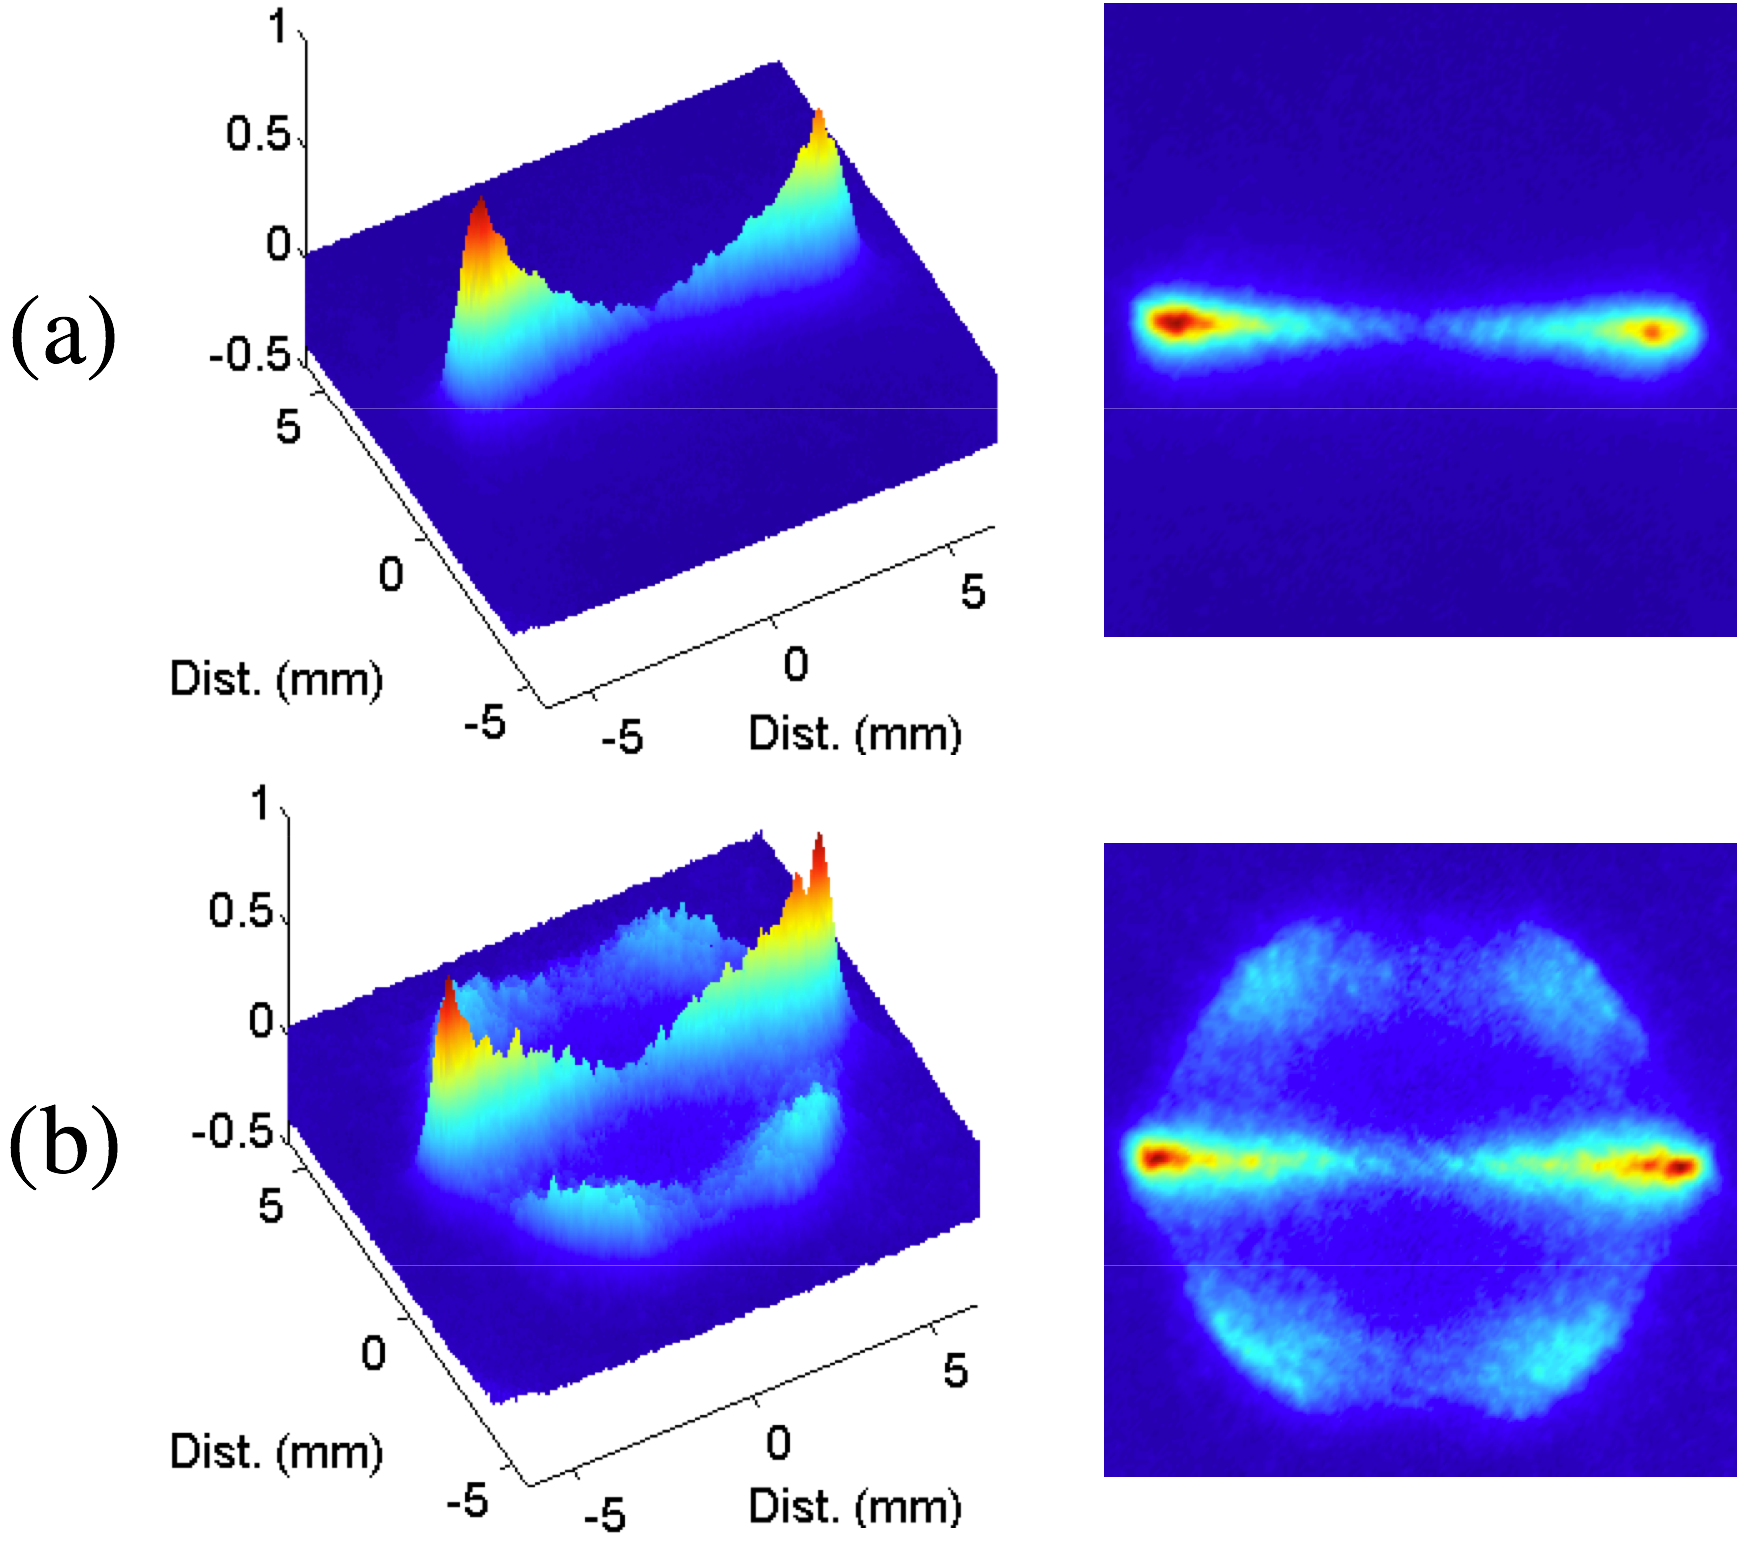
\includegraphics[height=3in]{ExperimentalResults}
    \caption{Experimental results. The difference between (a) and (b) is that the outcoupling Rabi frequency has been increased by an order of magnitude in (b).}
    \label{Peaks:ExperimentalResults}
\end{figure}

\begin{figure}
    \centering
        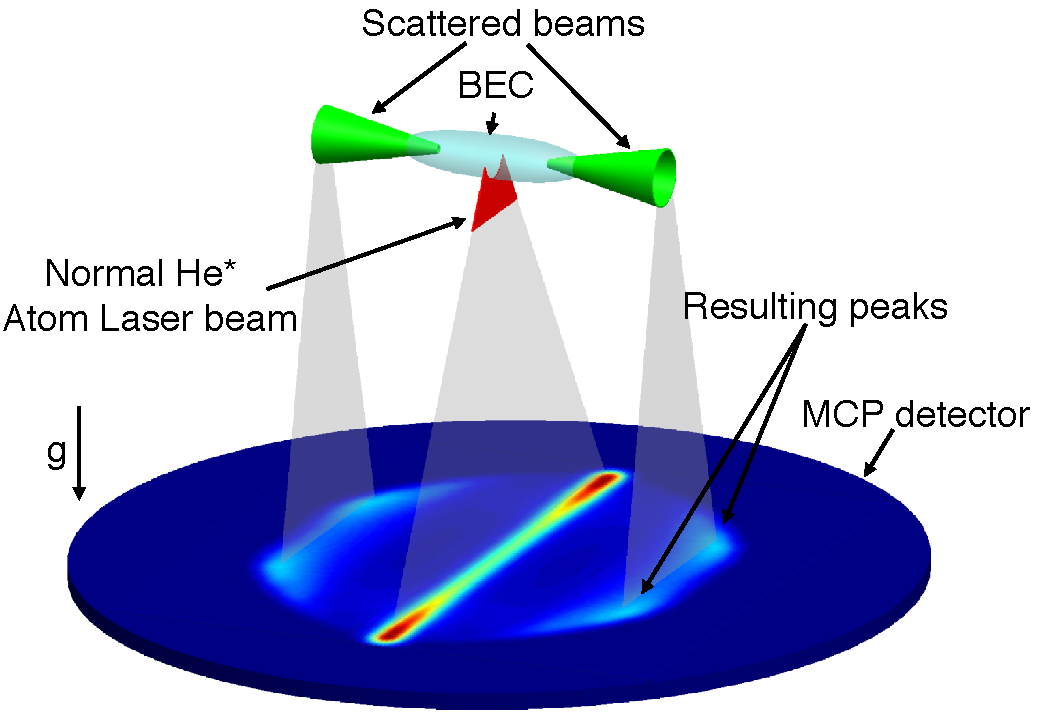
\includegraphics[height=3in]{Schematic}
    \caption{Schematic of the experimental setup}
    \label{Peaks:Schematic}
\end{figure}


\begin{table}
    \centering
    \begin{tabular}{cc}
    \toprule
    Parameter & Value\\
    \midrule
    Condensate number & $N = 2\times 10^6$\\
    Radial trapping frequency & $\omega_r = 2 \pi \times \unit[1020]{Hz}$\\
    Axial trapping frequency & $\omega_z = 2\pi \times \unit[55]{Hz}$\\
    Outcoupling Rabi frequency & $\Omega = 2\pi \times \unit[3]{kHz}$\\
    \bottomrule
    \end{tabular}
    \caption{Experimental parameters for the metastable Helium BEC under consideration.}
    \label{Peaks:ExperimentalParameters}
\end{table}

\section{Overview of Bogoliubov theory}
\label{Peaks:ElementaryExcitations}

The observed features in the atom laser profile presented in the previous section are caused by a dynamical instability in the condensate. The modes which are dynamically unstable are identified in the next section in which the excitation spectrum of the condensate is obtained. In this section an overview is given of the Bogoliubov theory which is used to obtain the excitation spectrum of the condensate and to determine its stability.

The problem is to determine the response of the condensate to small fluctuations about the mean-field. Typically the condensate is stable to such fluctuations, and their energy spectrum determines the phase and group velocities of the excitations.  In the case that the condensate is dynamically unstable some modes will undergo exponential growth, which corresponds to the generalised energy spectrum containing nonzero imaginary components. As a concrete example of the techniques demonstrated in this section, we consider a single-component condensate described by the Hamiltonian
\begin{align}
    \label{Peaks:ElementaryExcitationsExampleHamiltonian}
    \hat{H} &= \int d \bm{x}\, \hat{\Psi}^\dagger \left( -\frac{\hbar^2 \nabla^2}{2 M} + V(\bm{x}) + \frac{1}{2} U \hat{\Psi}^\dagger \hat{\Psi} - \mu \right) \hat{\Psi},
\end{align}
where an arbitrary energy offset $\mu$ has been included. This term is introduced for calculational reasons and has no physical influence on the Hamiltonian\footnote{The energy offset cannot affect any expectation values as particle-number is conserved and the influence of the energy offset is just a different physically meaningless energy offset for each total number.}. For the case of calculating the excitation spectrum of a ground state, the arbitrary energy offset $\mu$ will be identified as the condensate chemical potential.

The principal idea in finding the excitation spectrum of \eqref{Peaks:ElementaryExcitationsExampleHamiltonian} is to take advantage of the usefulness of the Gross-Pitaevskii equation in describing the mean-field of the condensate to enable the quantum-mechanical fluctuations about the mean-field to be considered. To this end the deviation operator $\delta \hat{\Psi} = \hat{\Psi} - \mean{\hat{\Psi}}$ is defined, and considered to be a small quantity\footnote{Although most easily understood in terms of spontaneously-broken symmetry (refer to \sectionref{BackgroundTheory:SymmetryBreaking}), this argument is true in general because the Hamiltonian $\hat{H}$ is unchanged by the global gauge transformation $\hat{\Psi}\mapsto\hat{\Psi}e^{i\phi}$. The results of the following calculation are therefore independent of the choice of $\phi$.}. The Hamiltonian \eqref{Peaks:ElementaryExcitationsExampleHamiltonian} can then be expanded in powers of $\delta \hat{\Psi}$,
\begin{align}
    \label{Peaks:HamiltonianPowerSeriesExpansion}
    \hat{H} &= \hat{H}_0 + \hat{H}_1 + \hat{H}_2 + \hat{H}_3 + \hat{H}_4.
\end{align}
The excitation spectrum of the Hamiltonian $\hat{H}$ is then approximately given by the eigenvalue spectrum of the lowest order nonzero term in \eqref{Peaks:HamiltonianPowerSeriesExpansion}.

The zeroth order term in \eqref{Peaks:HamiltonianPowerSeriesExpansion}
\begin{align}
    \hat{H}_0 &= \int d \bm{x}\, \mean{\hat{\Psi}}^* \left( -\frac{\hbar^2 \nabla^2}{2M} + V(\bm{x}) + \frac{1}{2} U \big|\mean{\hat{\Psi}}\big|^2 - \mu \right) \mean{\hat{\Psi}}
\end{align}
is simply a constant and represents the total energy of the unexcited mean-field. The first order term is of the form
\begin{align}
    \hat{H}_1 &= \int d \bm{x}\, \delta \hat{\Psi}^\dagger \left(i \hbar \frac{\partial \mean{\hat{\Psi}}}{\partial t} \right)  + \int d \bm{x}\, \left(i \hbar \frac{\partial \mean{\hat{\Psi}}}{\partial t} \right)^* \delta \hat{\Psi},
\end{align}
where the mean-field $\mean{\hat{\Psi}}$ evolves as
\begin{align}
    i \hbar \frac{\partial}{\partial t}\mean{\hat{\Psi}} &= \left(-\frac{\hbar^2 \nabla^2}{2 M} + V(\bm{x}) + U \big| \mean{\hat{\Psi}}\big|^2 - \mu \right) \mean{\hat{\Psi}}.
\end{align}
The first order term $\hat{H}_1$ does not affect the evolution of the deviation operator
\begin{align}
    i \hbar \frac{\partial }{\partial t}\hat{\Psi} &= \comm{\hat{\Psi}, \hat{H}}\\
    i \hbar \frac{\partial }{\partial t}\delta{\hat{\Psi}} + i \hbar \frac{\partial }{\partial t}\mean{\hat{\Psi}} &= \comm{\mean{\hat{\Psi}}, \hat{H}} + \comm{\delta\hat{\Psi}, \hat{H}}\\
    i \hbar \frac{\partial }{\partial t}\delta \hat{\Psi} &= \comm{\delta \hat{\Psi}, \hat{H}} - i \hbar \frac{\partial }{\partial t} \mean{\hat{\Psi}}\\
    &= \comm{\delta \hat{\Psi}, \hat{H}_1} + \comm{\delta \hat{\Psi}, \hat{H}_2 + \hat{H}_3 + \hat{H}_4} - i \hbar \frac{\partial }{\partial t}\mean{\hat{\Psi}}\\
    &= i \hbar \frac{\partial }{\partial t}\mean{\hat{\Psi}} + \comm{\delta \hat{\Psi}, \hat{H}_2 + \hat{H}_3 + \hat{H}_4} - i \hbar \frac{\partial }{\partial t}\mean{\hat{\Psi}}\\
    &= \comm{\delta \hat{\Psi}, \hat{H}_2 + \hat{H}_3 + \hat{H}_4}.
\end{align}
The first physically important term in \eqref{Peaks:HamiltonianPowerSeriesExpansion} is
\begin{align}
    \begin{split}
        \hat{H}_2 &= \int d \bm{x}\, \delta \hat{\Psi}^\dagger \left(-\frac{\hbar^2 \nabla^2}{2 M} + V(\bm{x}) + 2 U\big|\mean{\hat{\Psi}}\big|^2 -\mu \right)\delta\hat{\Psi}\\
         &\relphantom{=} + \frac{1}{2} U\int d \bm{x}\, \left(\mean{\hat{\Psi}}\mean{\hat{\Psi}} \delta \hat{\Psi}^\dagger\delta \hat{\Psi}^\dagger  +  \mean{\hat{\Psi}}^*\mean{\hat{\Psi}}^* \delta \hat{\Psi} \,\delta \hat{\Psi}\right).
    \end{split}
\end{align}
As the deviation operator $\delta \hat{\Psi}$ is small in some sense compared to the mean field $\mean{\hat{\Psi}}$, the higher-order contributions $\hat{H}_3$ and $\hat{H}_4$ to the total Hamiltonian can then be neglected compared to $\hat{H}_2$. The excitation spectrum of the condensate about the mean field $\mean{\hat{\Psi}}$ is then given by the energy spectrum of $\hat{H}_2$.

To avoid directly solving the infinite dimensional eigenvalue problem $\hat{H}_2 \ket{\Psi} = E \ket{\Psi}$ for the condensate excitation spectrum, it is desired to apply a linear transformation to $\hat{H}_2$ that will diagonalise it in the form
\begin{align}
    \label{Peaks:QuadraticHamiltonianAnsatz}
    \hat{H}_2 &= \sum_i \hbar \omega_i \hat{\Lambda}_i^\dagger \hat{\Lambda}_i^{\phantom{\dagger}},
\end{align}
for some boson annihilation operators $\hat{\Lambda}_i$ and real frequencies $\omega_i$. In this form, the Hamiltonian can be simply interpreted as representing a set of modes with energies $\hbar \omega_i$, which is the condensate excitation spectrum. The eigenvalues of $\hat{H}_2$ can also be identified as $\{n \hbar \omega_i : n > 0 \}$. It is not possible in general to transform $\hat{H}_2$ into the form \eqref{Peaks:QuadraticHamiltonianAnsatz} if the Hamiltonian possesses any instabilities \citep{Leonhardt:2003}, however one frequently considers the excitation spectrum of the ground state which is stable by definition and in this case such a transformation is always possible.

In the general case, we look for the operators $\hat{\Lambda}_i$ satisfying
\begin{align}
    \label{Peaks:ElementaryExcitationsEvolution}
    i \hbar \frac{\partial }{\partial t}\hat{\Lambda}_i &= \comm{\hat{\Lambda}_i, \hat{H}_2 } = - \hbar \omega_i \hat{\Lambda}_i
\end{align}
where $\omega_i$ is real if and only if $\hat{\Lambda}_i$ is a boson annihilation operator \citep{Leonhardt:2003}. In the case that $\omega_i$ is complex, boson annihilation operators can be constructed from the $\hat{\Lambda}_i$ as discussed in \appendixref{FloquetAppendix}. Hence $\hbar\omega_i$ can be considered to be a generalised energy spectrum of the condensate where nonzero imaginary components correspond to dynamical instabilities of the condensate. Note that although the eigenvalues of $\hat{H}_2$ must be real as it is hermitian, the eigenvalues of \eqref{Peaks:ElementaryExcitationsEvolution} need not be real. For example, the Hamiltonian for degenerate parametric amplification $\hat{H} = \hbar\chi \left(\hat{a}\hat{a} + \hat{a}^\dagger \hat{a}^\dagger \right)$ is hermitian but its eigenvalues in \eqref{Peaks:ElementaryExcitationsEvolution} are pure imaginary. In this case the occupation of the mode $\hat{a}$ undergoes exponential growth. The case of complex eigenvalues $\omega_i$ is discussed further in \sectionref{Peaks:ExperimentEigenvalues} and \appendixref{FloquetAppendix}.

Equation \eqref{Peaks:ElementaryExcitationsEvolution} is most easily solved by expanding the $\hat{\Lambda}_i$ in a complete, linearly independent basis $\{\hat{\Upsilon}_j\}$ such that $\hat{\Lambda}_i = \bm{c}_i^\dagger \hat{\bm{\Upsilon}}$ where $\bm{c}_i$ is a complex vector, $\bm{c}_i^\dagger$ denotes the conjugate-transpose, and $\hat{\bm{\Upsilon}}$ is the column vector formed by the complete basis $\{\hat{\Upsilon}_j\}$. As the Hamiltonian $\hat{H}_2$ is quadratic, its commutator with every operator $\hat{\Upsilon}_j$ will be linear in the operators $\{\hat{\Upsilon}_j\}$. Defining the complex matrix $\mathcal{H}$ to represent this relationship as
\begin{align}
    \label{Peaks:ScriptHRelationshipToHamiltonian}
    \sum_k \mathcal{H}_{jk} \hat{\Upsilon}_k &= \comm{\hat{\Upsilon}_j, \hat{H}_2}
\end{align}
permits \eqref{Peaks:ElementaryExcitationsEvolution} to be recast as an eigenvalue problem in $\mathcal{H}$,
\begin{align}
    \comm{\bm{c}_i^\dagger \hat{\bm{\Upsilon}}, \hat{H}_2} &= \bm{c}_i^\dagger \mathcal{H} \hat{\bm{\Upsilon}} = - \hbar \omega_i \bm{c}_i^\dagger \hat{\bm{\Upsilon}}, \label{Peaks:ElementaryExcitationsEigenvalueProblemWithOperators}\\
    \implies \bm{c}_i^\dagger \mathcal{H} &= - \hbar \omega_i \bm{c}_i^\dagger \label{Peaks:ElementaryExcitationsEigenvalueProblem}
\end{align}
where the last line follows as the components of $\hat{\bm{\Upsilon}}$ are linearly independent. If the mean-field $\mean{\hat{\Psi}}$ is time-independent, then the matrix $\mathcal{H}$ will also be time-independent and \eqref{Peaks:ElementaryExcitationsEigenvalueProblem} represents an eigenvalue problem for the left eigenvectors $\bm{c}_i^\dagger$ and eigenvalues $-\hbar \omega_i$ of the matrix $\mathcal{H}$. If the mean-field $\mean{\hat{\Psi}}$ simply evolves due to a global phase rotation, this can be cancelled by appropriate choice of the arbitrary energy offset $\mu$ making $\mathcal{H}$ time-independent.  In the case of the condensate ground state, that offset will be the chemical potential of the condensate. The eigenvalues $\{\hbar \omega_i\}$ then represent the generalised excitation spectrum of the condensate about the mean field, which was to be determined. 

It is important to note that for the eigenvalues of $\mathcal{H}$ to determine the solution to \eqref{Peaks:ElementaryExcitationsEvolution} the matrix $\mathcal{H}$ must be constant. In the next section these techniques will be generalised to the case of a \emph{periodic} mean-field in which the time-dependence of the matrix $\mathcal{H}$ cannot be removed by any analytic transformation.

In the case of a homogenous condensate ($V(\bm{x}) = 0$) the matrix $\mathcal{H}$ can be diagonalised analytically to give the condensate excitation spectrum as
\begin{align}
    \hbar \omega(\bm{k}) &= \sqrt{\varepsilon(\bm{k})\left(\varepsilon(\bm{k}) + 2 n U \right)},
    \label{Peaks:BogoliubovSpectrum}
\end{align}
where $\bm{k}$ is the wavevector, $\displaystyle \varepsilon(\bm{k}) = \frac{\hbar^2 \bm{k}^2}{2 M}$ is the free-particle energy spectrum and $n = \big|\mean{\hat{\Psi}} \big|^2$ is the condensate density. Equation~\eqref{Peaks:BogoliubovSpectrum} is known as the Bogoliubov energy spectrum \citep{Bogoliubov:1947}.

The interested reader is referred to the review paper by \citet{Ozeri:2005} for further details about Bogoliubov theory in Bose-Einstein condensates.

\section{Condensate excitations in the perturbative regime}
\label{Peaks:PerturbativeApproach}
%While the argument in the previous section gives a qualitative explanation for the four-wave mixing process observed in He*, it is not entirely satisfying. In this section an approximate analytic expression for the excited modes of the He* system will be obtained and investigated using Bogoliubov stuff.

The observed features in the atom laser profile presented in \sectionref{Peaks:ExperimentalSetup} are caused by a dynamical instability in the condensate that causes the formation of momentum excitations in a narrow range of momenta along the weak trapping axis. During outcoupling these excitations are accelerated along the tight trapping directions forming the momentum cones pictured in \figureref{Peaks:Schematic}. The detection process vertically integrates this momentum profile leading to the observed peaks in \figureref{Peaks:ExperimentalResults}.
% The background halo between these peaks and the usual atom laser profile is the result of (at higher detunings resonant momentum will vary across surfaces, during this initial switch-on phase, a range of momenta are excited)\footnote{FIXME: Complete and correct this sentence.}.

The dynamical instability is due to the significantly different scattering lengths between the Zeeman levels of He*. In a later section a full multimode quantum-field calculation will be discussed and its results presented, but it is enlightening to first consider a simplified model in which the energy spectrum (and stability) of small excitations to the condensate can be obtained.

The simplified model to be considered is that of a homogenous spinor condensate consisting of two levels with Rabi oscillations coupling the two levels. The approximation that the condensate is homogenous (known as the local density approximation \cite{Stamper-Kurn:1999,Zambelli:2000}) is justified if the excitations under considerations have wavelengths much smaller than the Thomas-Fermi radius in that dimension. The local density approximation will hold for this system along the axial direction as the axial momentum of the features observed in \figureref{Peaks:ExperimentalResults} corresponds to an excitation wavelength of $\sim \unit[5]{\micro m}$, significantly smaller than the Thomas-Fermi radius in the axial direction of $z_\text{TF} = \unit[175]{\micro m}$. 

The second approximation made in this model is to neglect the antitrapped state $m_F=-1$. Any density in this state leaves the condensate very rapidly due to the combined effects of both the mean-field repulsion and the magnetic field gradient. A classical particle in the centre of the condensate under the influence of the same effective potential experienced by the $m_F=-1$ atoms would reach a momentum equal to the momentum width of the condensate (and hence no longer be able to couple to the stationary atoms in the middle of the condensate) in $\sim\unit[80]{\micro s}$, significantly shorter than the inverse Rabi frequency of $\sim \unit[300]{\micro s}$.

With these approximations made, the Hamiltonian for this system is
\begin{align}
    \label{Peaks:InitialHamiltonian}
    \begin{split}
    \hat{H} &= \sum_i \int d\bm{x}\, \hat{\Psi}_i^\dagger \left(\frac{-\hbar^2 \nabla^2}{2 M} - \mu\right)\hat{\Psi}_i^{\phantom{\dagger}} + \frac{1}{2} \sum_{i j} U_{i j}\int d\bm{x}\, \hat{\Psi}_i^\dagger \hat{\Psi}_j^\dagger \hat{\Psi}_j^{\phantom{\dagger}} \hat{\Psi}_i^{\phantom{\dagger}}\\
            &\phantom{=} + \hbar \Omega \int d\bm{x}\, \left(\hat{\Psi}_1^\dagger \hat{\Psi}_0^{\phantom{\dagger}} + \hat{\Psi}_0^\dagger \hat{\Psi}_1^{\phantom{\dagger}}\right),
    \end{split}
\end{align}
where $U_{ij} = 4\pi \hbar^2 a_{ij}/M$ is the nonlinear interaction strength, $a_{ij}$ is the s-wave scattering length between internal states $i$ and $j$, $\Omega$ is the Rabi frequency which is taken to be real, and $\mu$ is an energy offset which has been included to cancel the global phase rotation which would otherwise be present. The equations of motion corresponding to this Hamiltonian are
\begin{subequations}
    \label{Peaks:OperatorEquationsOfMotion}
    \begin{align}
    i \hbar \frac{\partial }{\partial t}\hat{\Psi}_1  &= -\frac{\hbar^2}{2M}\nabla^2 \hat{\Psi}_1  + U \left(\hat{\Psi}_1^\dagger \hat{\Psi}_1^{\phantom{\dagger}} + \hat{\Psi}_0^\dagger \hat{\Psi}_0^{\phantom{\dagger}}\right) \hat{\Psi}_1 + \hbar \Omega \hat{\Psi}_0 - \mu \hat{\Psi}_1,  \\
    i \hbar \frac{\partial }{\partial t}\hat{\Psi}_0 &= -\frac{\hbar^2}{2M} \nabla^2 \hat{\Psi}_0 + U \left(\hat{\Psi}_1^\dagger \hat{\Psi}_1^{\phantom{\dagger}} + \kappa \hat{\Psi}_0^\dagger \hat{\Psi}_0^{\phantom{\dagger}} \right) \hat{\Psi}_0 + \hbar \Omega \hat{\Psi}_1 - \mu \hat{\Psi}_0,
    \end{align}
\end{subequations}
where $U=U_{11}=U_{10}$ and $\kappa = U_{00}/U_{11}$. For metastable Helium in the $F=1$ manifold, $\protect{\kappa \approx 0.74}$\footnote{FIXME: Cite something.}, while for Rubidium in the $F=1$ manifold, $\kappa \approx 1.01$ \cite{Ho:1998}\footnote{FIXME: A more recent reference might be useful.}. 

\subsection{The dynamical steady-state}
\label{Peaks:MeanFieldPeriodicity}

The excitation spectrum of a condensate can be obtained by approximating each field operator to be a c-number (the mean-field) plus a small fluctuation term, and then either diagonalising the Hamiltonian \cite{Bogoliubov:1947,FetterWalecka} or diagonalising the linearised equations of motion for the fluctuations themselves (see \sectionref{Peaks:ElementaryExcitations}). It is the latter approach that will be taken here, but with the difference that the mean-field about which the linearisation procedure will take place is itself \emph{time-dependent}.

The mean-field state that we wish to consider is one that corresponds to the state of the BEC in the experiment. At $t=0$ all of the population in this state will be in the $m_F=1$ level, representing the original trapped BEC, while the $m_F=0$ atom laser level will be initially unpopulated. Rabi oscillations will transfer population between these two levels, and it will be shown that these oscillations are periodic.

The method for diagonalising the evolution equations of the linearised fluctuations to obtain the excitation spectrum is the same method used to determine the stability of fixed points of systems of nonlinear ordinary differential equations. As mentioned in the previous section, this method relies critically on the fact that it is a stationary solution about which the equations are linearised. Floquet's Theorem \citep{Nayfeh:1995} allows the stability of \emph{periodic} solutions to be considered, and it is this theorem that will be used to determine the stability of the condensate about these mean-field dynamics. It will now be shown that the mean-field evolution of \eqref{Peaks:OperatorEquationsOfMotion} is periodic.

Within the local density approximation we can assume that the mean-field remains homogeneous; only the excitations will have spatial dependence. The equations of motion for the mean-field then reduce to the following ordinary differential equations,
\begin{subequations}
    \label{Peaks:MeanFieldEquationsOfMotion}
    \begin{align}
    i \hbar \frac{d }{dt}\Psi_1 &= U\left(\abs{\Psi_1}^2 + \abs{\Psi_0}^2\right)\Psi_1 + \hbar \Omega \Psi_0 - \mu \Psi_1,\\
    i \hbar \frac{d }{dt}\Psi_0 &= U\left(\abs{\Psi_1}^2 + \kappa \abs{\Psi_0}^2\right)\Psi_0 + \hbar \Omega \Psi_1 - \mu \Psi_0.
    \end{align}
\end{subequations}

Although solving \eqref{Peaks:MeanFieldEquationsOfMotion} for $\kappa \neq 1$ is intractable analytically, it can at least be shown that the solutions are periodic up to a global phase rotation, and exactly periodic for appropriate choice of the arbitrary energy offset $\mu$. This can be shown by recognising these equations as modified optical Bloch equations containing a nonlinear term but with no damping. Defining $\Psi_i = c_i\sqrt{n}$ where $n = \abs{\Psi_1}^2 + \abs{\Psi_0}^2$ is the total density, the equations of motion for the density matrix terms $\rho_{10} = c_{1}^{}c_{0}^*$ and $w = \rho_{11}-\rho_{00} = \abs{c_1}^2 - \abs{c_0}^2$ are
\begin{subequations}
    \label{Peaks:OpticalBlochEquations}
    \begin{align}
        \frac{d}{dt}\rho_{10} &= -i\frac{g}{2} (1-w)\rho_{10} + i \Omega w,\\
        \frac{d }{dt}w &= -4 \Omega \Im\{\rho_{10}\},
    \end{align}
\end{subequations}
where $g = n U (1-\kappa)/\hbar$. As the evolution is purely Hamiltonian, these equations will conserve the energy of the state. Up to an arbitrary additive constant, the energy per particle is given by
\begin{align}
    E &= -\frac{1}{8}\hbar g(1 - w)^2 + 2 \hbar \Omega \Re\{\rho_{10}\}.
    \label{Peaks:OpticalBlochEnergy}
\end{align}
The solutions to \eqref{Peaks:OpticalBlochEquations} are visualised in \figureref{Peaks:BlochSphere}.

As the evolution is purely Hamiltonian, the state can be described by a point on the surface of the Bloch sphere (see \figureref{Peaks:BlochSphere}).  The state is however not completely free to move on this sphere as the Hamiltonian must be conserved by its motion. This further restricts the system's motion to closed lines on the surface of the Bloch sphere, therefore requiring the system's motion to be periodic. Although this demonstrates that all physical expectation values are periodic as they must be independent of the global phase\footnote{It is the invariance of the Hamiltonian and hence all observables to a global phase rotation $\hat{\Psi} \rightarrow \hat{\Psi}e^{i \phi}$ that guarantees the conservation of atom number by Noether's theorem \citep{Noether:1918}.}, the global phase rotation must be cancelled. This can be achieved by appropriate choice of the energy offset $\mu$. It is the periodicity of the wavefunctions $\Psi_i$ that will enable the stability of the condensate to excitations to be determined.

\begin{figure}
    \centering
    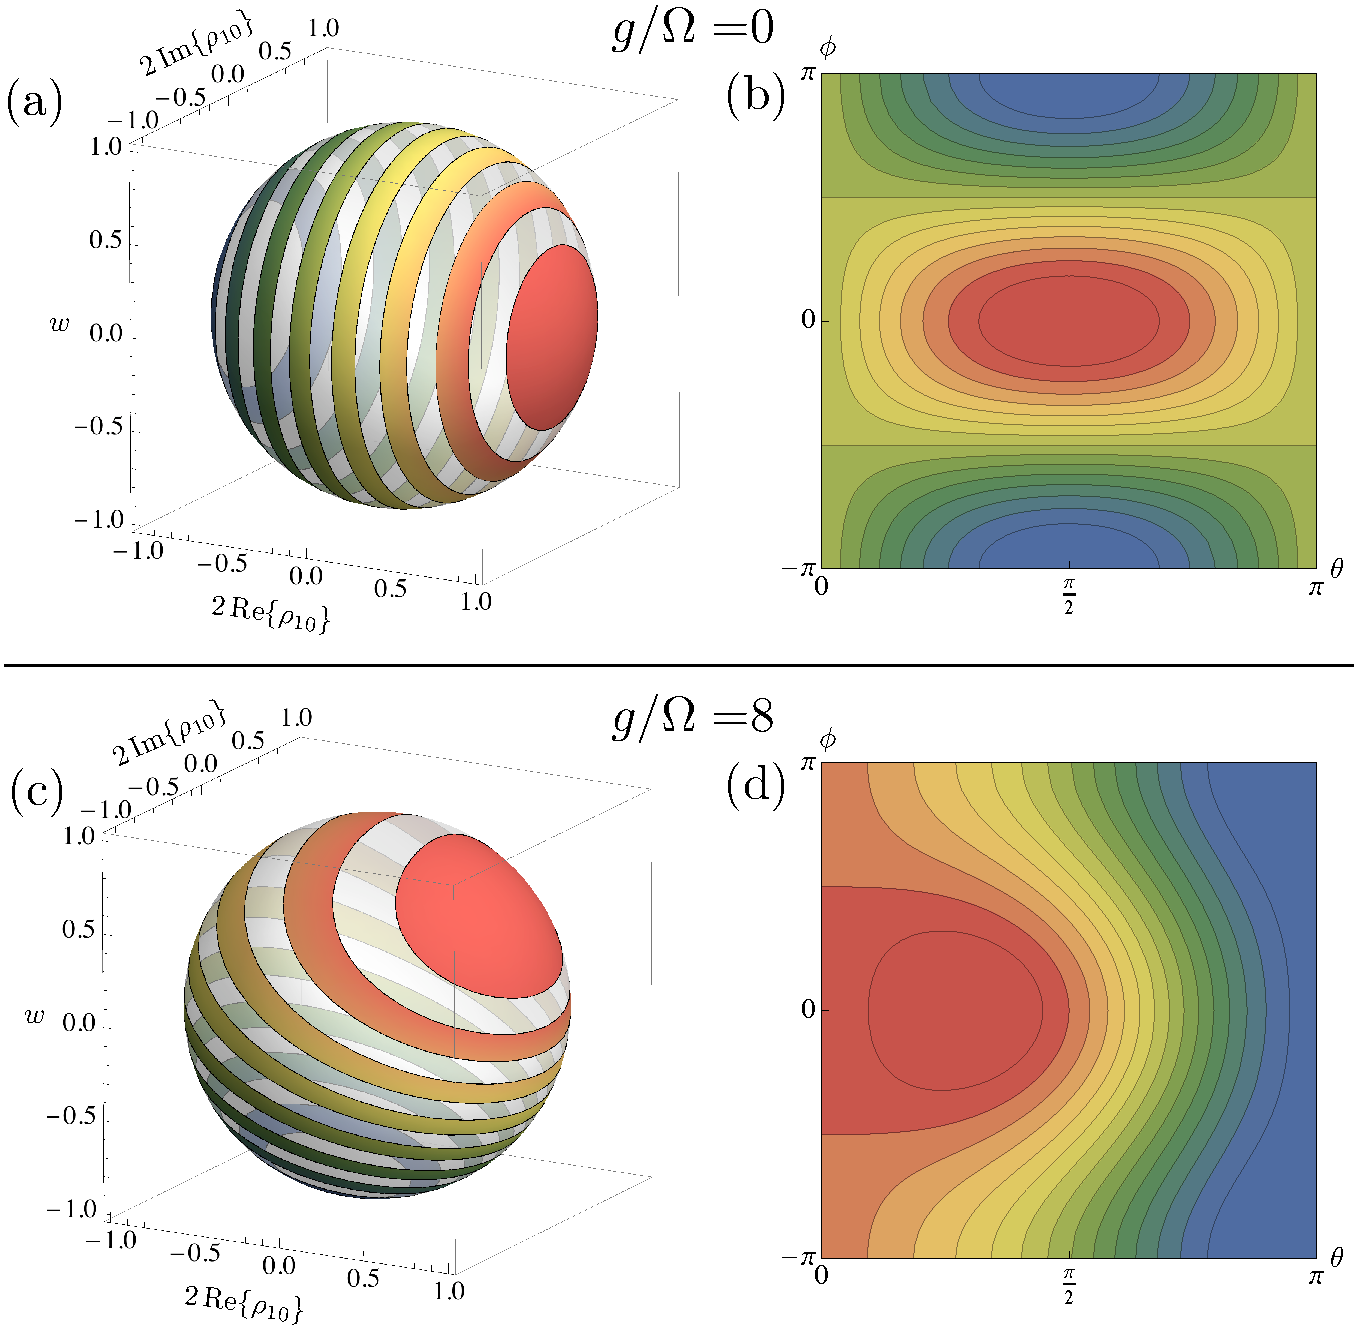
\includegraphics[width=14cm]{BlochSpheres}
    \caption{Bloch sphere representation of the evolution described by \eqref{Peaks:OpticalBlochEquations}. The upper figures (a) and (b) represent the case of the usual optical Bloch equations with no damping ($g/\Omega=0$), the lower figures (c) and (d) illustrate the effect of the nonlinear term on the evolution with $g/\Omega = 8$. The left figures (a) and (c) illustrate the Bloch sphere coloured according to the energy $E$ [see~\eqref{Peaks:OpticalBlochEnergy}]. The system is constrained to move on lines of constant colour. Bands have been removed from these spheres for illustration purposes only. The right figures (b) and (d) are contour plots of the energy $E$ over the surface of the Bloch sphere.
     \label{Peaks:BlochSphere}}
\end{figure}

\subsection{Excitation dynamics}

The evolution of small perturbations about the mean-field dynamics of a condensate define both the excitation spectrum of the condensate and its stability to perturbations. 
%These perturbations not only arise from experimental uncertainties, but are an  inescapable consequence of quantum mechanics due to the fluctuations of the vacuum itself.
To determine the evolution of these excitations the mean-field dynamics must be separated from that of the excitations. To this aim we define the deviation operators $\delta\hat{\Psi}_i = \hat{\Psi}_i - \mean{\hat{\Psi}_i}$ and treat $\delta\hat{\Psi}_i$ as a small quantity. In this case the $\mean{\hat{\Psi}_i}=\Psi_i$ are themselves time dependent, obeying the equations for the mean-field \eqref{Peaks:MeanFieldEquationsOfMotion}.

The equations of motion for the deviation operators are obtained by replacing the field operators $\hat{\Psi}_i$ in the operator evolution equations \eqref{Peaks:OperatorEquationsOfMotion} with $\Psi_i + \delta \hat{\Psi}_i$ and keeping only terms up to first order in the deviation operators. Applying this procedure gives
\begin{subequations}
    \label{Peaks:DeviationOperatorsEvolutionXSpace}
    \begin{align}
        \begin{split}
            i \hbar \frac{\partial }{\partial t}\delta \hat{\Psi}_1 =& U\left[ \left(2\abs{\Psi_1}^2+\abs{\Psi_0}^2 \right)\delta \hat{\Psi}_1 + \Psi_1^2\delta\hat{\Psi}_1^\dagger + \Psi_1\Psi_0\delta\hat{\Psi}_0^\dagger + \Psi_0^*\Psi_1\delta\hat{\Psi}_0\right]\\
                    & - \frac{\hbar^2}{2M}\nabla^2 \delta \hat{\Psi}_1 +\hbar \Omega\delta\hat{\Psi}_0- \mu \delta \hat{\Psi}_1,
        \end{split}\\
        \begin{split}
        i \hbar \frac{\partial }{\partial t}\delta \hat{\Psi}_0 =& U\left[\left(2\kappa \abs{\Psi_0}^2 +\abs{\Psi_1}^2\right)\delta\hat{\Psi}_0 + \kappa \Psi_0^2 \delta\hat{\Psi}_0^\dagger + \Psi_1\Psi_0\delta\hat{\Psi}_1^\dagger + \Psi_1^*\Psi_0\delta\hat{\Psi}_1\right]\\
                    & -\frac{\hbar^2}{2M}\nabla^2 \delta \hat{\Psi}_0 +\hbar \Omega\delta\hat{\Psi}_1 - \mu \delta\hat{\Psi}_0.
        \end{split}
    \end{align}
\end{subequations}

Having assumed the mean-field to be homogenous, the evolution equations are spatially translation-invariant and will take their simplest form in a Fourier basis. Performing the Fourier transform of \eqref{Peaks:DeviationOperatorsEvolutionXSpace} yields
\begin{subequations}
    \label{Peaks:DeviationOperatorsEvolutionKSpace}
    \begin{align}
        \begin{split}
            i \hbar \frac{\partial }{\partial t}\delta \hat{\Psi}_1(\bm{k}) =& U\left[ \left(2\abs{\Psi_1}^2+\abs{\Psi_0}^2 \right)\delta \hat{\Psi}_1(\bm{k}) + \Psi_1^2\delta\hat{\Psi}_1^\dagger(-\bm{k}) + \Psi_1\Psi_0\delta\hat{\Psi}_0^\dagger(-\bm{k}) + \Psi_0^*\Psi_1\delta\hat{\Psi}_0(\bm{k})\right]\\
                    & +\frac{\hbar^2 \bm{k}^2}{2M} \delta \hat{\Psi}_1(\bm{k}) +\hbar \Omega\delta\hat{\Psi}_0(\bm{k})- \mu \delta \hat{\Psi}_1(\bm{k}),
        \end{split}\\
        \begin{split}
        i \hbar \frac{\partial}{\partial t} \delta \hat{\Psi}_0(\bm{k}) =& U\left[\left(2\kappa \abs{\Psi_0}^2 +\abs{\Psi_1}^2\right)\delta\hat{\Psi}_0(\bm{k}) + \kappa \Psi_0^2 \delta\hat{\Psi}_0^\dagger(-\bm{k}) + \Psi_1\Psi_0\delta\hat{\Psi}_1^\dagger(-\bm{k}) + \Psi_1^*\Psi_0\delta\hat{\Psi}_1(\bm{k})\right]\\
                    & +\frac{\hbar^2 \bm{k}^2}{2M} \delta \hat{\Psi}_0(\bm{k}) +\hbar \Omega\delta\hat{\Psi}_1(\bm{k}) - \mu \delta\hat{\Psi}_0(\bm{k}).
        \end{split}
    \end{align}
\end{subequations}

In this form, it is clear that the Fourier modes are almost completely decoupled from each other. Each deviation operator $\delta\hat{\Psi}_i(\bm{k})$ is only coupled to $\left\{\delta\hat{\Psi}_j(\bm{k}),\, \delta\hat{\Psi}_j^\dagger(-\bm{k})\right\}$, with each $\delta\hat{\Psi}_i^\dagger(-\bm{k})$ also only coupled to this same set. This can be exploited to write the equations \eqref{Peaks:DeviationOperatorsEvolutionKSpace} in matrix form as
\begin{align}
    \label{Peaks:DeviationOperatorsMatrixEvolution}
    i \hbar \frac{\partial }{\partial t}\hat{\bm{\Upsilon}}(\bm{k}) &= \mathcal{H}(\bm{k}) \hat{\bm{\Upsilon}}(\bm{k}),
\end{align}
where
\begin{align}
    \hat{\bm{\Upsilon}}(\bm{k}) &= 
    \begin{pmatrix}
        \delta\hat{\Psi}_1(\bm{k}) &
        \delta\hat{\Psi}_1^\dagger(-\bm{k}) &
        \delta\hat{\Psi}_0(\bm{k}) &
        \delta\hat{\Psi}_0^\dagger(-\bm{k})
    \end{pmatrix}^\text{T},\\
    \mathcal{H}(\bm{k}) &= 
    \begin{pmatrix}
        \varepsilon(\bm{k}) + q_{1} - \mu & v_{11} & u_{01} + \hbar \Omega & v_{10}\\
        -v_{11}^* & -\varepsilon(\bm{k}) - q_1 + \mu & -v_{10}^* & -u_{10} - \hbar \Omega\\
        u_{10} + \hbar \Omega & v_{10} & \varepsilon(\bm{k}) + q_0 - \mu & \kappa v_{00}\\
        -v_{10}^* & -u_{01} - \hbar \Omega & -\kappa v_{00}^* & -\varepsilon(\bm{k}) - q_0 + \mu
    \end{pmatrix},\label{Peaks:HMatrix}
\end{align}
and $q_1 = U\left(2\abs{\Psi_1}^2+\abs{\Psi_0}^2\right)$, $q_0 = U\left(2\kappa \abs{\Psi_0}^2 + \abs{\Psi_1}^2\right)$, $u_{ij} = U\Psi_i^*\Psi_j$, $v_{ij} = U\Psi_i\Psi_j$, and $\displaystyle \protect{\varepsilon(\bm{k}) = \frac{\hbar^2 \bm{k}^2}{2M}}$.

Note that the matrix $\mathcal{H}(\bm{k})$ is not the Hamiltonian, but is related to it by \eqref{Peaks:ScriptHRelationshipToHamiltonian}. As a consequence, although it will be shown later that in some circumstances $\mathcal{H}(\bm{k})$ contains complex eigenvalues and is hence not hermitian this in no way conflicts with the requirement that the Hamiltonian $\hat{H}$ must be hermitian and only have real eigenvalues.

If the coefficients of the matrix $\mathcal{H}(\bm{k})$ were not time-dependent, the excitation spectrum of the condensate could simply be obtained from the eigenvalues of $\mathcal{H}(\bm{k})$. Non-zero imaginary components for these eigenvalues would indicate the corresponding mode to be unstable. Before continuing with the general case of $\kappa \neq 1$, in the next section the limit in which all scattering lengths are equal ($\kappa=1$) will be considered and some familiar results recovered.

\subsection{Excitation spectra in the $\kappa = 1$ limit}
\label{Peaks:Kappa1Limit}
In the limit that all the scattering lengths are the same ($\kappa = 1$), the nonlinear term in \eqref{Peaks:MeanFieldEquationsOfMotion} only contributes to a rotation of the global phase of the spinor condensate. In this case the dynamics can be solved analytically and familiar excitation spectra recovered.

The general solution to \eqref{Peaks:MeanFieldEquationsOfMotion} for $\kappa = 1$ is
\begin{subequations}
    \label{Peaks:Kappa1MeanFieldSolution}
    \begin{align}
        \Psi_1(t) &= \cos(\Omega t) \Phi_+ + \sin(\Omega t) \Phi_-, \\
        \Psi_0(t) &= -i\sin(\Omega t) \Phi_+ + i\cos(\Omega t) \Phi_-,
    \end{align}
\end{subequations}
for some complex constants $\Phi_\pm$, and where the chemical potential $\mu = n U$ has cancelled the global phase rotation. This solution can be viewed as a linear basis transformation from $\hat{\Psi}_i$ to $\hat{\Phi}_\pm$, which are the eigenvectors of the Rabi coupling term in \eqref{Peaks:InitialHamiltonian}. Performing this change of basis on the original Hamiltonian \eqref{Peaks:InitialHamiltonian} yields a Hamiltonian of the same form, but without the Rabi coupling term. The equations of motion for the deviation operators $\delta\hat{\Phi}_\pm$ therefore give a matrix of precisely the same form as \eqref{Peaks:HMatrix} but in terms of $\Phi_\pm$ and $\delta\hat{\Phi}_\pm$ instead of the $\Psi_i$ and $\delta\hat{\Psi}_i$, and with $\Omega$ replaced by 0. This new matrix $\mathcal{H}'(\bm{k})$ is time-independent and can be diagonalised to give the eigenvalues
\begin{subequations}
    \label{Peaks:Kappa1Eigenvalues}
    \begin{align}
        \hbar \omega_\uparrow(\bm{k}) &= \sqrt{\varepsilon(\bm{k})\left(\varepsilon(\bm{k}) + 2 n U\right)},\\
        \hbar \omega_\downarrow(\bm{k}) &= \varepsilon(\bm{k}),
    \end{align}
\end{subequations}
where $\displaystyle\varepsilon(\bm{k}) = \frac{\hbar^2\bm{k}^2}{2M}$, $n= \abs{\Psi_1}^2 + \abs{\Psi_0}^2$ and the remaining two eigenvalues are the negatives of \eqref{Peaks:Kappa1Eigenvalues}. $\hbar \omega_\uparrow(\bm{k})$ is the usual Bogoliubov spectrum \citep{Bogoliubov:1947} corresponding to excitations in the total condensate density. The eigenvalue $\hbar \omega_\downarrow(\bm{k})$ is the free particle spectrum; this excitation only changes the relative densities of the two states without affecting the total density, hence not affecting the nonlinear term in the Hamiltonian \eqref{Peaks:InitialHamiltonian}.

The Hamiltonian for the condensate excitations that corresponds to the eigenvalues \eqref{Peaks:Kappa1Eigenvalues} is (refer to \sectionref{Peaks:ElementaryExcitations})
\begin{align}
    \hat{H} &= \sum_{i=\uparrow,\downarrow}\int d\bm{k}\, \hbar \omega_i(\bm{k}) \hat{\Lambda}_i^\dagger(\bm{k}) \hat{\Lambda}_i^{\phantom{\dagger}}(\bm{k}),
\end{align}
where the $\hat{\Lambda}_{\uparrow,\downarrow}(\bm{k})$ obey boson commutation relations and are the corresponding normalised eigenvectors to the eigenvalues in \eqref{Peaks:Kappa1Eigenvalues}. The normalised eigenvectors for the negatives of those eigenvalues are the $\hat{\Lambda}_{\uparrow, \downarrow}^\dagger(-\bm{k})$.

\subsection[Floquet's theorem]{Floquet's theorem \citep{Nayfeh:1995}}
\label{Peaks:FloquetsTheorem}

Having considered the limit of equal scattering lengths, it now remains to determine the energy spectrum and condensate stability in the general case of $\kappa \neq 1$. Analytic results cannot be obtained in this limit, but numeric results corresponding to the experimental situation in \sectionref{Peaks:ExperimentalSetup} can be obtained.

In the general case, the excitation spectrum cannot be obtained from the eigenvalues of the matrix $\mathcal{H}(\bm{k})$ in \eqref{Peaks:HMatrix} as the matrix's entries are  themselves time-dependent. However, due to the periodicity of the mean-field wavefunctions demonstrated in \sectionref{Peaks:MeanFieldPeriodicity}, the entries of $\mathcal{H}(\bm{k})$ are themselves periodic, which enables Floquet's theorem to be applied.

Floquet's theorem proves that the matrix solution to the initial-value problem
\begin{subequations}
    \label{Peaks:FloquetMatrixIVP}
    \begin{align}
        \frac{d}{dt}\bm{\Pi}(t) &= \bm{A}(t) \bm{\Pi}(t),\\
        \bm{\Pi}(0) &= \mathbb{I},
    \end{align}
\end{subequations}
where $\mathbb{I}$ is the $n \times n$ identity matrix and $\bm{A}(t)$ a periodic $n \times n$ matrix with period $T$ can be written in the form
\begin{align}
    \bm{\Pi}(t) = \bm{P}(t) \exp(\bm{Q} t),
\end{align}
for some constant matrix $\bm{Q}$ and $\bm{P}(t)$ a matrix function with period $T$ and $\bm{P}(0) = \mathbb{I}$. The matrix solution $\bm{\Pi}(t)$ is the general solution to the related linear system
\begin{align}
    \frac{d}{dt}\bm{x}(t) &= \bm{A}(t) \bm{x}(t),
    \label{Peaks:FloquetVectorIVP}
\end{align}
for any initial condition $\bm{x}(0)$ where $\bm{x}(t)$ is a vector. Every solution $\bm{x}(t)$ to this problem can be written in terms of the matrix $\bm{\Pi}(t)$ as
\begin{align}
    \bm{x}(t) &= \bm{\Pi}(t) \bm{x}(0),
\end{align}
as is easily verified. The matrix solution $\bm{\Pi}(t)$ thus completely determines the behaviour of all solutions to \eqref{Peaks:FloquetVectorIVP}.

The eigenvalues of $\bm{Q}$ are known as \emph{Floquet exponents} (or \emph{characteristic exponents}) and determine the long-term growth or decay of the solutions to \eqref{Peaks:FloquetVectorIVP}. These eigenvalues can be obtained from the \emph{monodromy matrix},
\begin{align}
    \label{Peaks:MonodromyMatrix}
    \mathcal{M} &= \bm{\Pi}(T) = \exp(\bm{Q} T),
\end{align}
as $\bm{P}(T) = \bm{P}(0) = \mathbb{I}$. The existence and uniqueness of the solution to \eqref{Peaks:FloquetMatrixIVP} guarantees that $\bm{\Pi}(t)$ and hence $\mathcal{M}$ will be invertible. The Floquet exponents $\xi_i$ can therefore be obtained from the eigenvalues $\lambda_i$ of the monodromy matrix using $\lambda_i = \exp(\xi_i T)$. It is the Floquet exponents of the matrix $\mathcal{H}(\bm{k})$ that we wish to calculate in order to determine the stability of the condensate to excitations.

\subsection{Determination of the dynamical instabilities}
\label{Peaks:ExperimentEigenvalues}

The method outlined in the previous section for determining the Floquet exponents of the system \eqref{Peaks:DeviationOperatorsMatrixEvolution} requires knowledge of its period $T$, and hence the period of the mean field dynamics given by \eqref{Peaks:MeanFieldEquationsOfMotion}. Although this period cannot be determined analytically, it can be found numerically.

It was shown in \sectionref{Peaks:MeanFieldPeriodicity} that up to a global phase rotation $\displaystyle f(T) = e^{i 2\pi \Delta \nu T}f(0)$, the mean fields $\Psi_j(t)$ are periodic. The mean fields $\Psi_j(t)$ can be therefore written in the form
\begin{align}
    \label{Peaks:MeanFieldFourierDecomposition}
    \Psi_j(t) = \sum_{n=-\infty}^\infty \alpha_{j,n} \exp\left[i 2\pi \left( n \nu_0 + \Delta\nu\right)t \right],
\end{align}
for some complex constants $\alpha_{j, n}$, fundamental frequency $\nu_0 = T^{-1}$, and frequency offset $\Delta \nu$. In this form, the $\Psi_j(t)$ are not exactly periodic as $\Psi_j(T) = \exp(i\Delta \nu T)\Psi_j(0)$, but this frequency offset can be cancelled by an appropriate choice of the energy offset $\mu = 2\pi\hbar \Delta \nu$ in \eqref{Peaks:InitialHamiltonian}.

The period $T$ and frequency offset $\Delta\nu$ in \eqref{Peaks:MeanFieldFourierDecomposition} can be determined from the Fourier transform of $\Psi_j(t)$ which will have sharp peaks at the frequencies $n \nu_0 + \Delta \nu$ (see \figureref{Peaks:MeanFieldFourierTransform}). Choosing the energy offset $\mu=-h \nu$, the frequency offset in \eqref{Peaks:MeanFieldFourierDecomposition} can be cancelled making the $\Psi_j(t)$ with this energy offset exactly periodic with period $T$. \figureref{Peaks:MeanFieldFourierTransform} illustrates the Fourier transform of the numerical solutions for $\Psi_j(t)$ for a Rabi frequency of $\Omega = 2 \pi \times \unit[3]{kHz}$ from which the period $T=\unit[150]{\micro{}s}$ and frequency offset $\Delta \nu = \unit[-1.78]{kHz}$ have been obtained.

\begin{figure}
    \centering
    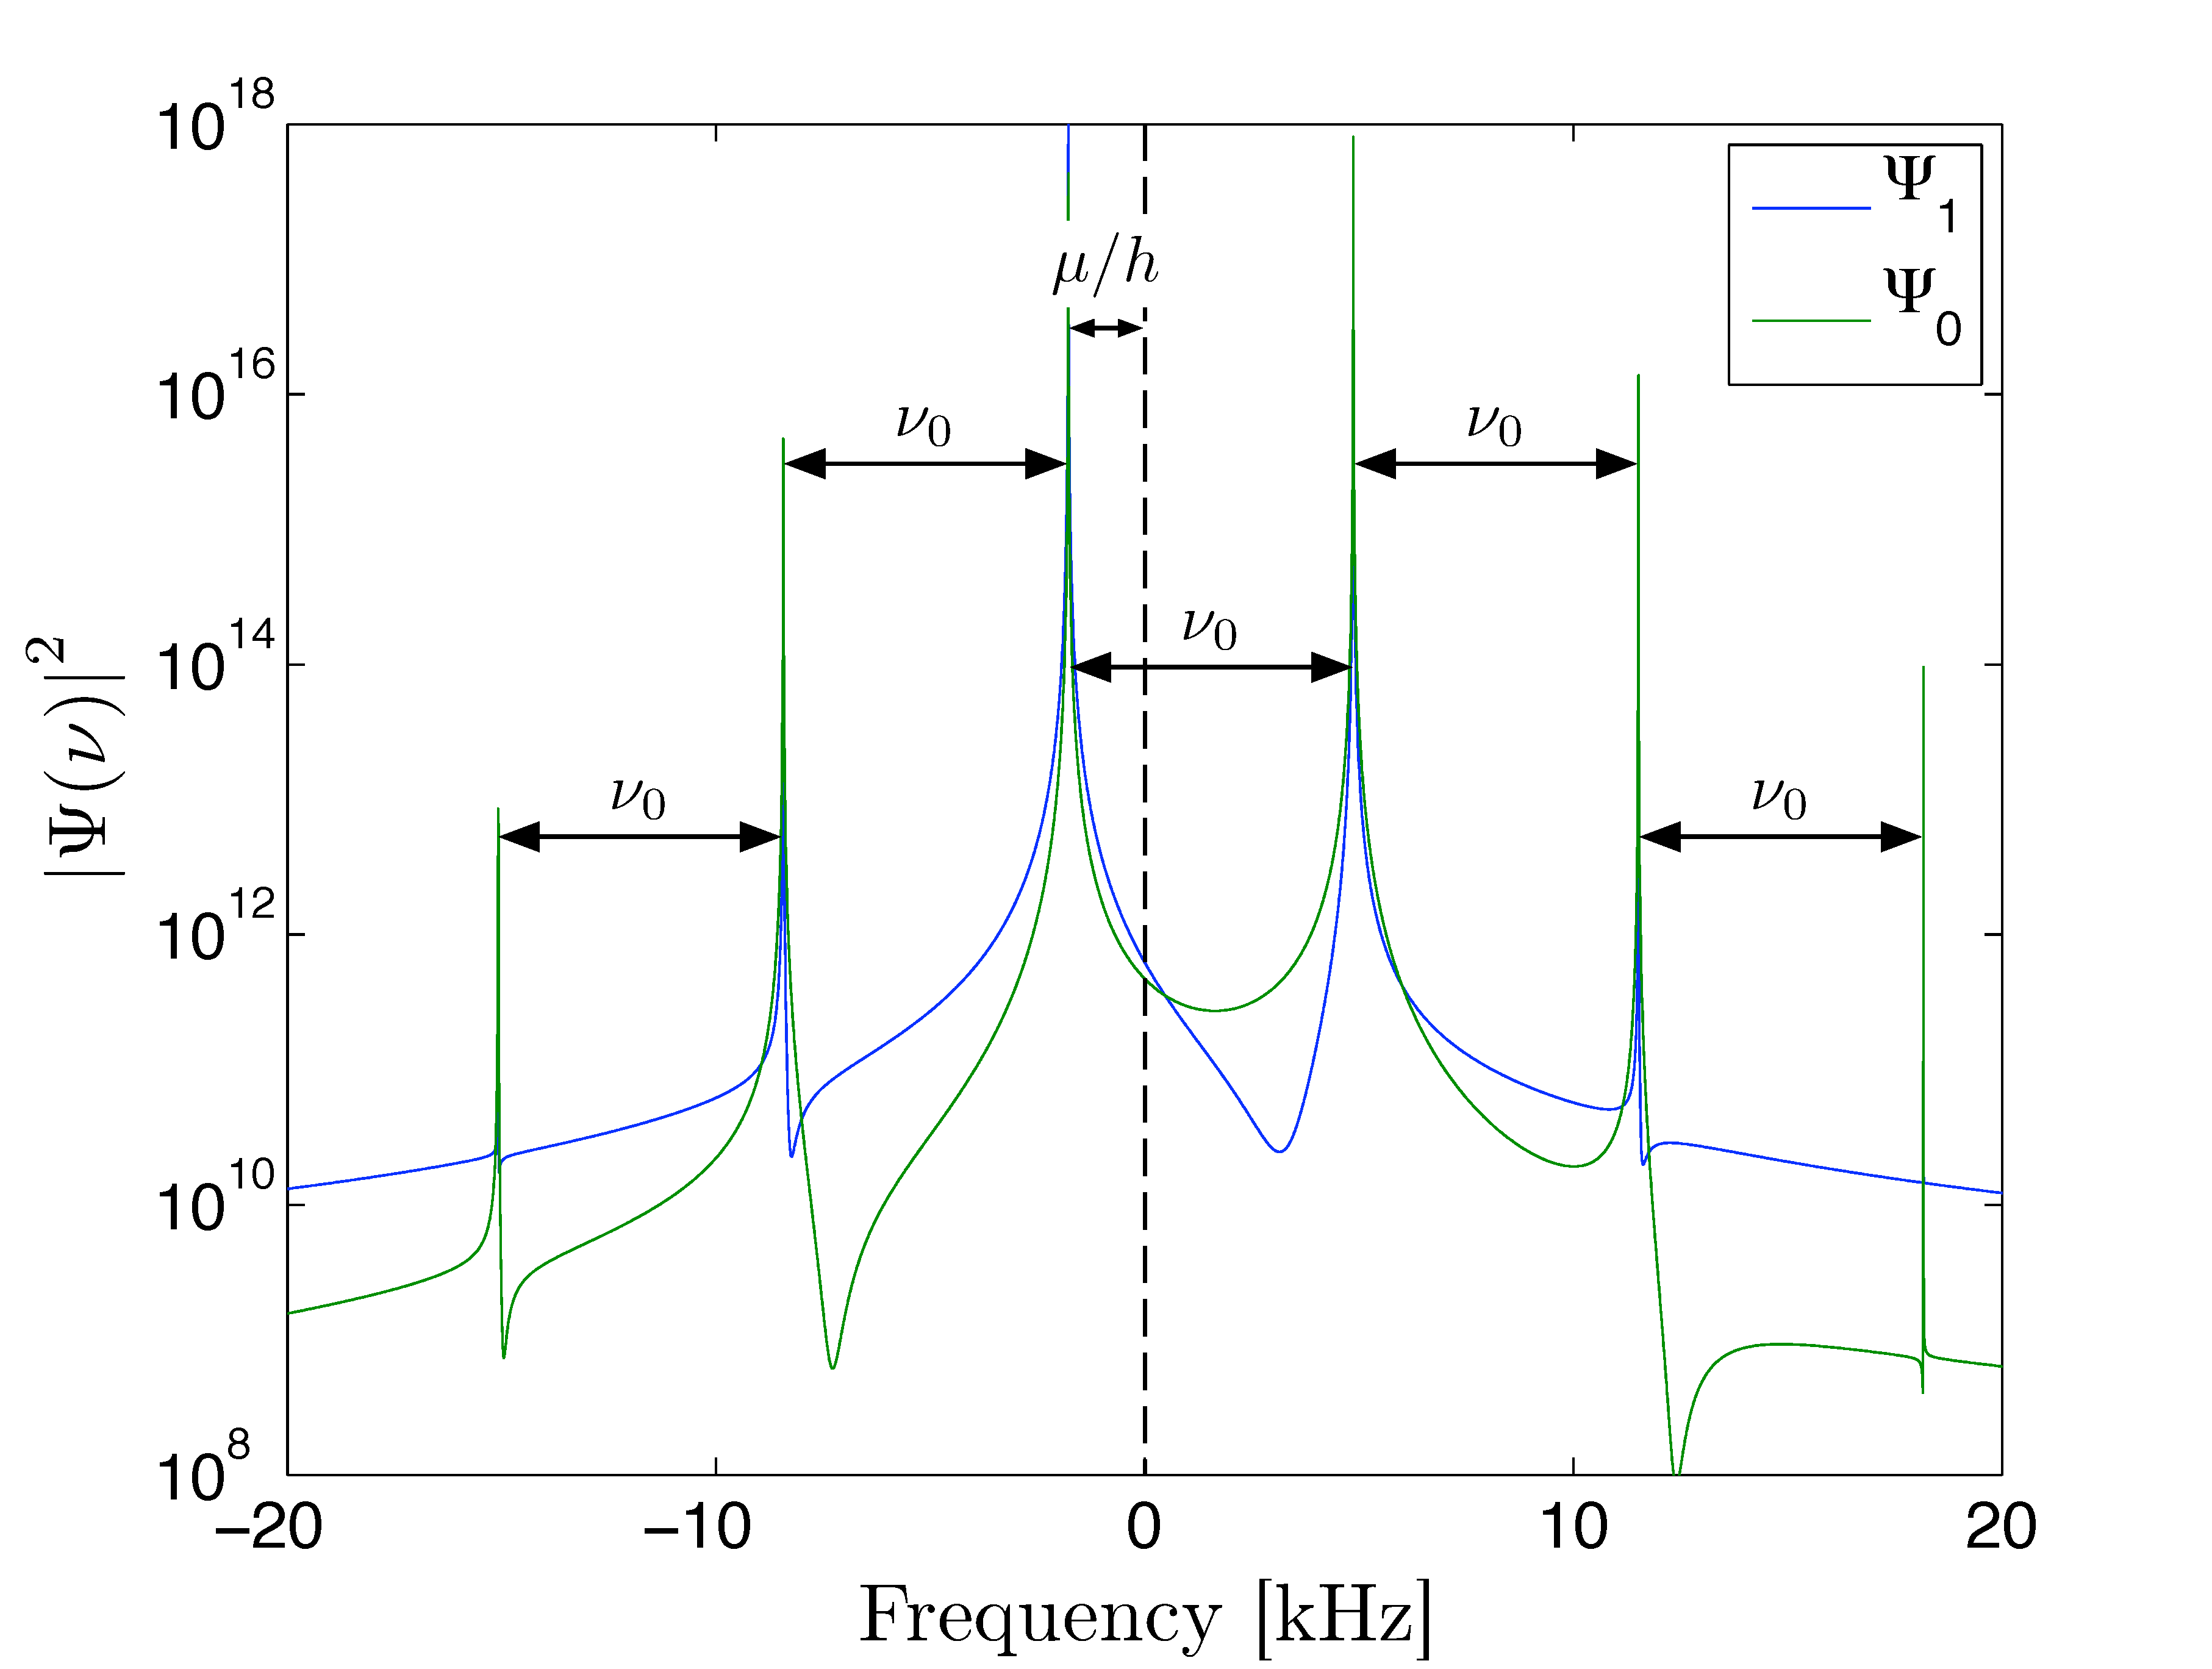
\includegraphics[width=14cm]{MeanFieldFourierTransform}
    \caption{\label{Peaks:MeanFieldFourierTransform} Temporal Fourier transform of the calculated mean field evolution defined by \eqref{Peaks:MeanFieldEquationsOfMotion} for the centre of the condensate defined by the experimental parameters given in \tableref{Peaks:ExperimentalParameters}. The frequency $\nu_0$ is the inverse period of the system, and $\Delta\nu$ represents the global phase rotation. From the data in this figure the values $\nu_0 = \unit[6.65]{kHz}$ and $\Delta\nu = \unit[-1.78]{kHz}$ can be determined, giving the period as $T=\unit[150]{\micro{}s}$.}
\end{figure}

The period and energy offset determined, it remains to calculate the mono\-dromy matrix $\mathcal{M}(\bm{k})$ from which the Floquet exponents may be derived. This is achieved by numerically solving the related matrix problem to \eqref{Peaks:DeviationOperatorsMatrixEvolution} from $t=0$ to $t=T$ [refer to \eqref{Peaks:MonodromyMatrix}]. Noting that the matrix $\mathcal{H}(\bm{k})$ only depends on $k = \abs{\bm{k}}$, the solutions for the Floquet exponents $\xi(\bm{k}) = \gamma(\bm{k}) + i\omega(\bm{k})$ are illustrated in \figureref{Peaks:CondensateEigenvalues}.

In the limit that the mean-field is time-independent (a degenerate case of periodicity), the Floquet exponents $\xi(\bm{k})$ are related to the eigenvalues $\lambda(\bm{k})$ of the matrix $\mathcal{H}$ by $\xi(\bm{k}) = \frac{-i}{\hbar} \lambda(\bm{k})$. It was previously stated that eigenvalues of $\mathcal{H}(\bm{k})$ with nonzero imaginary components would be unstable, this therefore corresponds to having a nonzero \emph{real} component of the Floquet exponent $\xi(\bm{k})$.

\begin{figure}
    \centering
    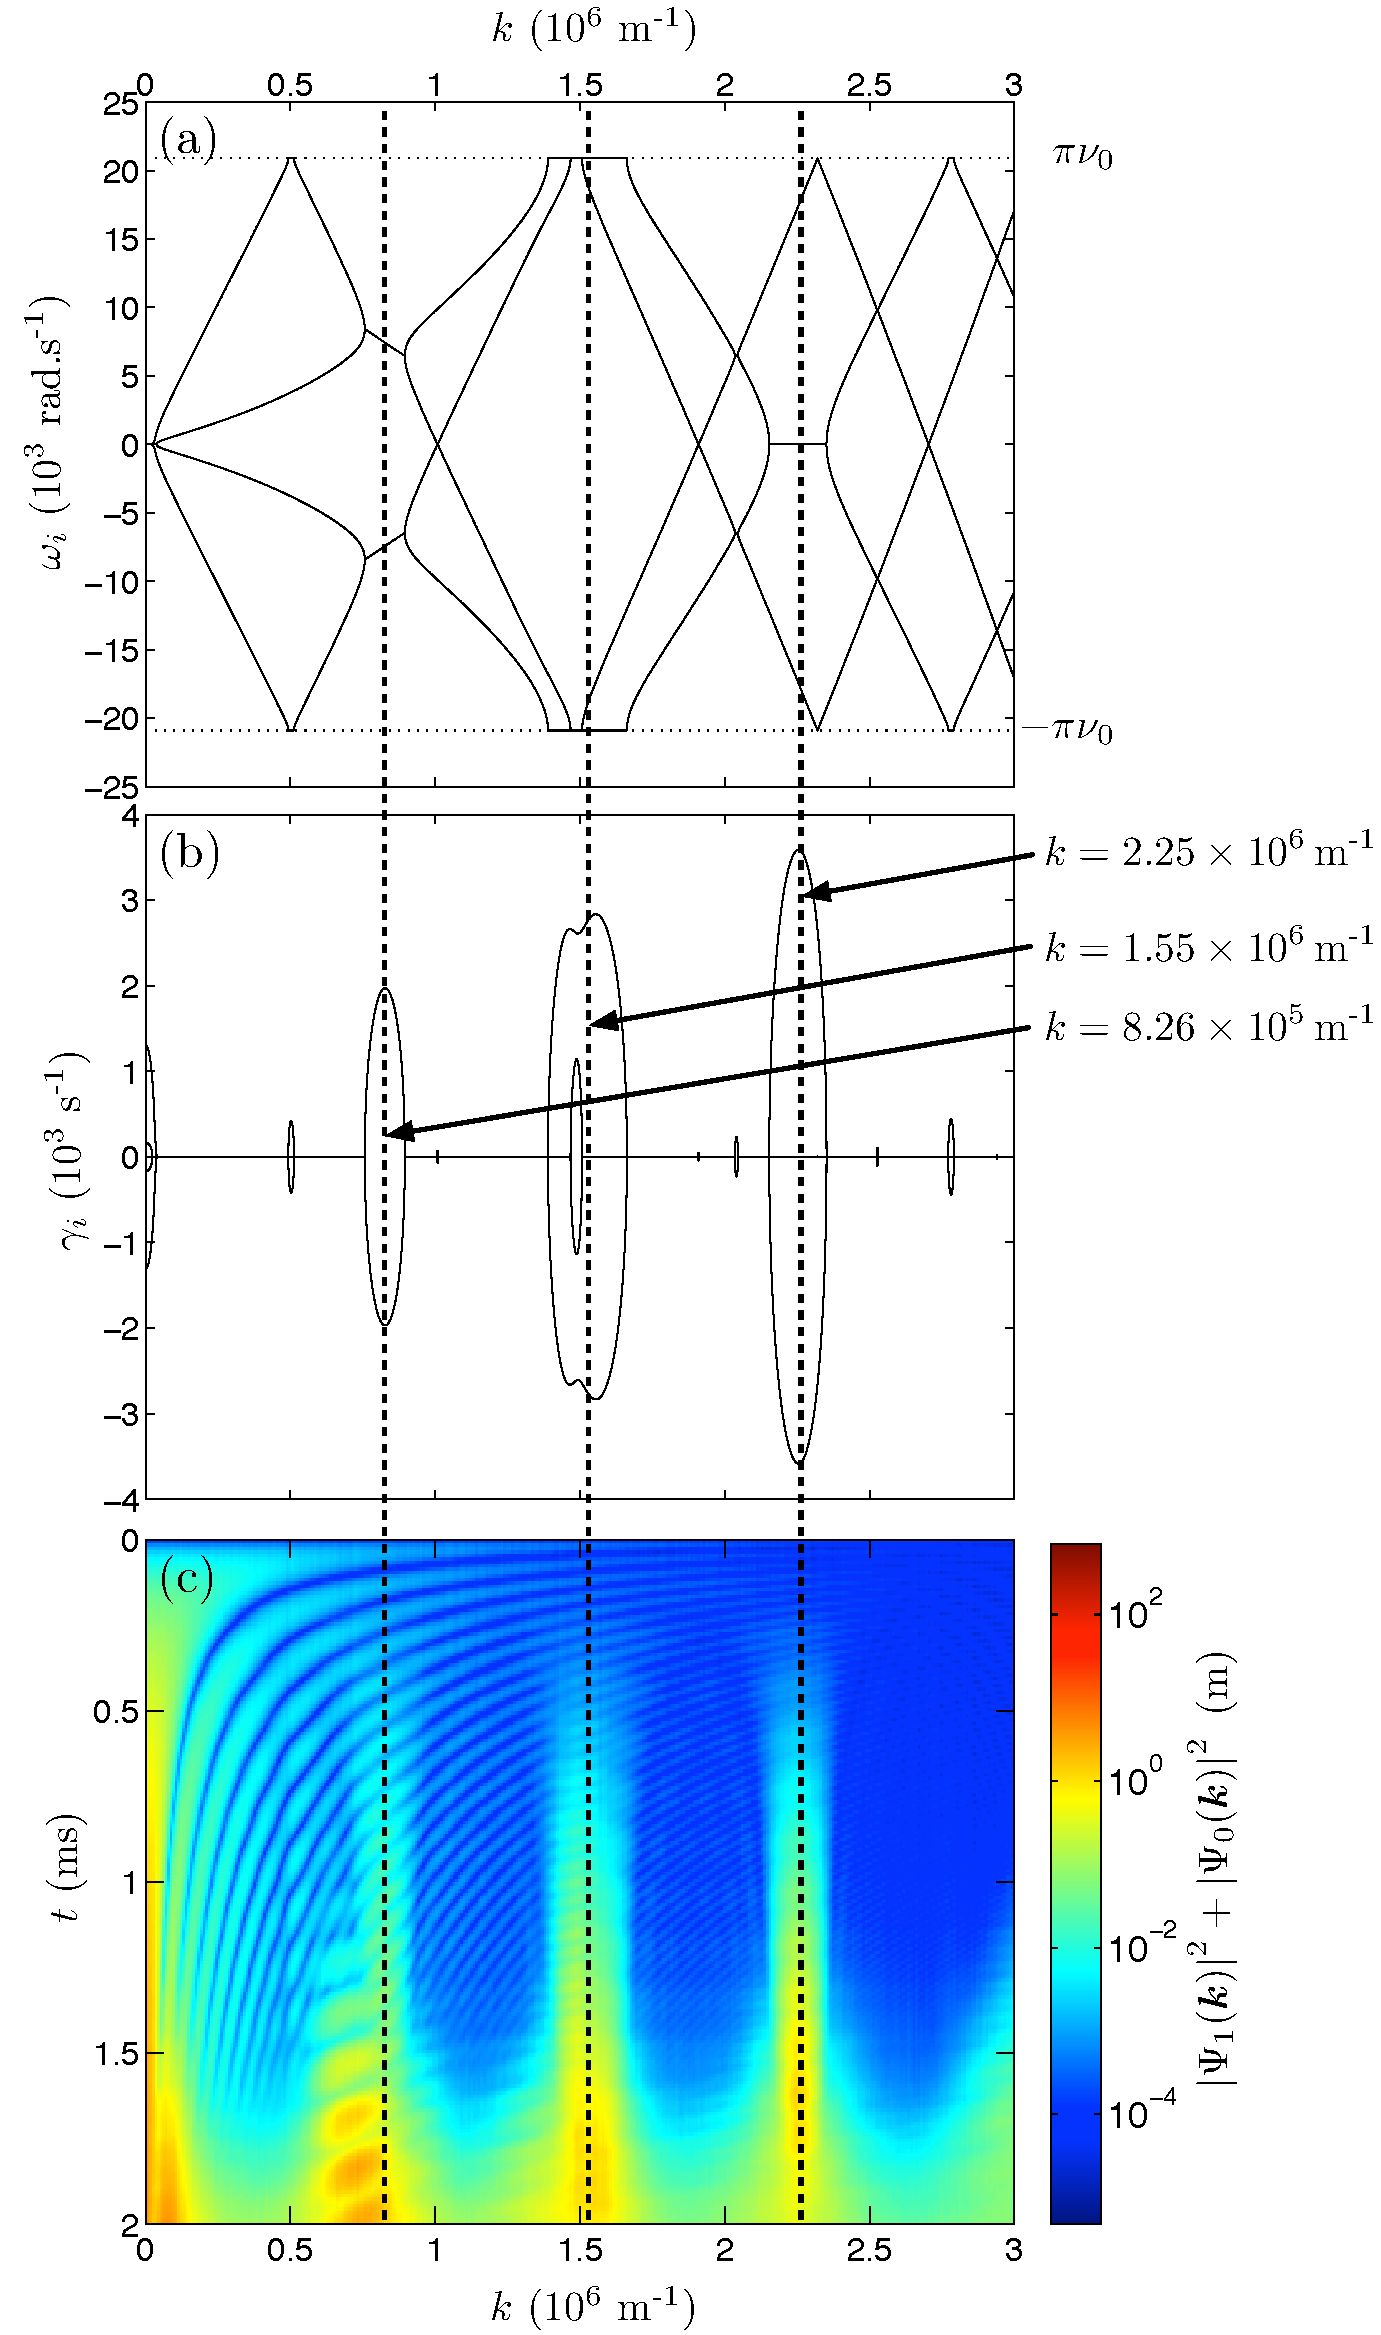
\includegraphics[height=19cm]{CondensateEigenvalues}
    \caption{\label{Peaks:CondensateEigenvalues}
        Illustration of the Floquet exponents for $\mathcal{H}(\bm{k})$ and comparison to a corresponding truncated Wigner simulation for $\Omega = 2\pi \times \unit[3]{kHz}$.
        Upper figure (a) displays the imaginary part $\omega_i$ of the Floquet exponents. As the $\omega_i$ can only be determined up to a multiple of $2\pi\nu_0$ [see \eqref{Peaks:AmbiguityFloquetExponent}], they have been reduced modulo $2\pi\nu_0$ into the range $\left[-\pi\nu_0,\, \pi\nu_0\right]$.
        The middle figure (b) shows the real part $\gamma_i$ of the Floquet exponents, which indicate an instability for the corresponding wavenumber when they are nonzero.
        Lower figure (c) shows the results of a 1D truncated Wigner simulation corresponding to the system under consideration in (a) and (b). The truncated Wigner simulation exhibits growth in the same modes predicted from the results of the perturbative analysis shown in (b). The truncated Wigner results shown are the average of 500 paths.}
\end{figure}

The temporal periodicity of the system implies that the imaginary components $\omega_i(\bm{k})$ of the Floquet exponents are only uniquely defined modulo $2\pi \nu_0$ (see \figureref{Peaks:CondensateEigenvalues}(a)). This is because any eigenvalue $\lambda$ of the monodromy matrix $\mathcal{M}(\bm{k})$ corresponds to infinitely many Floquet exponents,
\begin{align}
    \label{Peaks:AmbiguityFloquetExponent}
    \lambda = \exp\left[\left(\gamma + i\omega + i 2 \pi n \nu_0\right)T\right] = \exp\left[\left(\gamma + i \omega\right)T\right].
\end{align}
This does not hinder our understanding of the system as our primary interest is in the stability of the condensate to excitations, which is determined by the $\gamma_i(\bm{k})$.

The normalised eigenvectors of the system are not always annihilation or creation operators; as is discussed in \appendixref{FloquetAppendix}, this is only true when the Floquet exponents are pure imaginary. When the Floquet exponents have a nonzero real component, annihilation and creation operators can be constructed from linear combinations of the eigenvectors. Not being eigenvectors, these operators will therefore have nontrivial evolution. As is shown in \appendixref{FloquetAppendix}, Floquet exponents with nonzero real parts come in pairs of the form $\pm \gamma(\bm{k}) + i \omega(\bm{k})$. From the corresponding eigenvectors to these Floquet exponents the bosonic annihilation operator $\hat{\Lambda}(\bm{k}, t)$ can be formed, which evolves as
\begin{subequations}
    \label{Peaks:DynamicalInstability}
    \begin{align}
        \hat{\Lambda}(\bm{k}, nT) &= e^{i n\omega(\bm{k}) T} \left( \sinh(n\gamma(\bm{k}) T) \hat{\Lambda}'^\dagger(-\bm{k}, 0) + \cosh(n\gamma(\bm{k}) T) \hat{\Lambda}(\bm{k}, 0)\right),\\
        \hat{\Lambda}'(\bm{k}, nT) &= e^{-i n \omega(\bm{k}) T} \left( \sinh(n\gamma(\bm{k}) T) \hat{\Lambda}^\dagger(-\bm{k}, 0) + \cosh(n\gamma(\bm{k}) T) \hat{\Lambda}'(\bm{k}, 0)\right),
    \end{align}
\end{subequations}
where $n$ is a positive integer, and where $\hat{\Lambda}'(\bm{k}, t)$ will be equal to $\hat{\Lambda}(\bm{k}, t)$ in some circumstances as discussed in \appendixref{FloquetAppendix}. Due to the exponential growth in \eqref{Peaks:DynamicalInstability}, the mode corresponding to $\hat{\Lambda}(\bm{k})$ represents a dynamical instability of the condensate.

The behaviour of the dynamical instabilities will be governed by \eqref{Peaks:DynamicalInstability} only while the unstable modes have a small occupation compared to the condensate, and scattering between the unstable modes can be neglected. \figureref{Peaks:CondensateEigenvalues}(c) shows the results of a truncated Wigner simulation of the Hamiltonian \eqref{Peaks:InitialHamiltonian}, which is in excellent agreement with the location of the dynamical instabilities as determined by the Floquet exponents [see \figureref{Peaks:CondensateEigenvalues}(b)]. For later times, there is an additional mode undergoing growth, $k \approx \unit[7.5\times 10^5]{m}^{-1}$. This mode is the result of scattering between the dynamical instabilities, a process neglected the perturbative approach taken in this section. 

\parasep

In summary, the procedure used to find the Floquet exponents of $\mathcal{H}(\bm{k})$, and hence the stability of the condensate to excitations is:
\begin{enumerate}
    \item Numerically solve \eqref{Peaks:MeanFieldEquationsOfMotion} with $\mu=0$ for a long period of time $t \gg T$ where $T$ is the periodicity of the solution.
    \item Perform the temporal Fourier transform of the solutions obtained for $\Psi_i(t)$ to accurately determine the period $T$ and the value of the energy offset $\mu$ required to cancel any global phase evolution to make the wavefunctions themselves periodic (see \figureref{Peaks:MeanFieldFourierTransform}).
    \item Using the calculated period and energy offset, numerically solve the related matrix problem to \eqref{Peaks:DeviationOperatorsMatrixEvolution} for a range of values of $\bm{k}$ to obtain the monodromy matrix $\mathcal{M}(\bm{k})$. In this calculation the matrix $\bm{A}(t)$ in \eqref{Peaks:FloquetMatrixIVP} is $\displaystyle -\frac{i}{\hbar}\mathcal{H}(\bm{k}, t)$.
    \item Calculate the eigenvalues $\lambda_i$ of $\mathcal{M}(\bm{k})$ and determine the Floquet exponents $\xi_i$ using $\protect{\lambda_i = \exp(\xi_i T)}$ (see \figureref{Peaks:CondensateEigenvalues}). The imaginary parts of these Floquet exponents gives the energy spectrum, with nonzero real parts giving the growth rate for the corresponding instability.
\end{enumerate}

\subsection{Discussion of the dynamical instabilities}

The evolution of the dynamical instability $\hat{\Lambda}(\bm{k})$ given by \eqref{Peaks:DynamicalInstability} is equivalent to that of the non-degenerate parametric amplifier \citep{WallsMilburn}, which is a model for the parametric down-conversion of light by a non-linear crystal. In parametric down-conversion, two EPR\footnote{FIXME: EPR entanglement will need to be defined somewhere} entangled photons are produced at frequencies $\omega_1$ and $\omega_2$ with growth rate $\gamma$ from a classical seed beam at frequency $\omega = \omega_1 + \omega_2$. Analogously, in the case of the He* BEC discussed at the start of this chapter the evolution represented by \eqref{Peaks:DynamicalInstability} will result in the spontaneous formation of EPR entangled pairs of excitations, one in each of the $\hat{\Lambda}(\pm \bm{k})$ modes. Although these modes will be entangled upon production, it does not necessarily follow that parts of the outcoupled atom laser will be entangled; the entangled $\hat{\Lambda}(\bm{k})$ modes are each superpositions of $m_F=1$ and $m_F=0$ states, but only the $m_F=0$ atoms can leave the condensate. However, if the $m_F=1$ components of the entangled modes are assumed to be outcoupled faster than the time to reverse their momenta ($\unit[9]{ms}$), then number difference squeezing between the atom laser components with opposite axial momenta may be observed.

These excitations would not necessarily be expected to form along the tight trapping directions. Of the three most unstable modes in \figureref{Peaks:CondensateEigenvalues}, the shortest wavelength for these excitations is $\lambda \approx \unit[3]{\micro m}$ which is not significantly smaller than the Thomas-Fermi radius in this dimension of $\rho_\text{TF} = \unit[9.4]{\micro m}$. Hence the local density approximation will not be satisfied in this dimension as the condensate density decays to zero over this distance. However, as the Thomas-Fermi radius in the axial dimension is $z_\text{TF} = \unit[175]{\micro m}$, the local density approximation will be a good approximation for describing the excitations along that dimension.

This effect also depends on the scattering length for collisions between $m_F=0$ atoms being significantly smaller than both the 1--1 and 1--0 scattering lengths as no instabilities were found in the $\kappa = 1$ limit (see \sectionref{Peaks:Kappa1Limit}). 
Consequently, this effect would not be expected to be observed in atoms like $\nucl{87}{}{Rb}$.

Verification that the $\hat{\Lambda}(\bm{k})$ quasiparticles are the origin of the peak-like structure observed in the experiment required a full 3D field calculation, which is discussed in \sectionref{Peaks:3DCalculation}.  The argument made in this section that the observed structure is due to the formation of pairs of quasiparticles formed via a spontaneous four-wave mixing process indicate that a Gross-Pitaevskii model will be unable to reproduce the observations. Such a mean-field model will be insufficient due to the absence of the vacuum fluctuations which are critical to all spontaneous processes.

It should be remarked at this point that if this behaviour was to be used to produce EPR entanglement, one would want to perform an experiment in the blah parameter regime.


\section{Full 3D calculation}
\label{Peaks:3DCalculation}
In the previous section it was found that the process of outcoupling from the He* BEC discussed in \sectionref{Peaks:ExperimentalSetup} results in certain modes within the condensate becoming unstable. It was argued that these instabilities will be the original cause of the observed structure in \figureref{Peaks:ExperimentalResults}. However, it is not immediately clear that these instabilities will not be suppressed by Penning ionisation which causes $m_F=0$ atoms to ionise but not samples of just $m_F=1$ atoms. To verify that the instabilities are not suppressed and that they do cause the observed structure, a detailed numerical simulation of the experiment was performed.

The master equation that describes the experiment described in \sectionref{Peaks:ExperimentalSetup} is given by
\begin{align}
    \label{Peaks:MasterEquation}
    \frac{d }{d t}\hat{\rho} &= \frac{-i}{\hbar} [\hat{H},\, \hat{\rho} ] + \frac{9}{2} K^\text{(unpol)}_{^{4}\text{He}} \int d \bm{x}\, \mathcal{D}\left[\hat{\Xi}_{S=0,m_S=0} \right] \hat{\rho},
\end{align}
where $\displaystyle\hat{\Xi}_{S, m_S}$ is the annihilation operator for the quasimolecular state with total hyperfine spin $S$ and projection $m_S$, $\mathcal{D}[\hat{c}]\hat{\rho} \equiv \hat{c}\hat{\rho}\hat{c}^\dagger - \frac{1}{2}(\hat{c}^\dagger \hat{c} \hat{\rho} + \hat{\rho} \hat{c}^\dagger \hat{c})$ is the usual decoherence superoperator, and the second term\footnote{The reason for the difference between the $\displaystyle \frac{54}{5}$ factor in \citet{Dall:2009} and \eqref{Peaks:MasterEquation} is a difference of a factor of $\sqrt{2}$ in the definitions of $\hat{\Psi}_{J=0}^{\text{(mol)}}$ in \citep{Dall:2009} and $\displaystyle\hat{\Xi}_\ket{S=0, m_S=0}$ here, and a calculational error of the order of 20\% in \citep{Dall:2009}.} on the RHS in \eqref{Peaks:MasterEquation} is due to Penning ionisation (refer to \sectionref{BackgroundTheory:Helium} and \appendixref{PenningIonisationAppendix}) with $K^\text{(unpol)}_{^{4}\text{He}}=\unit[7.7\times 10^{-17}]{m\textsuperscript{3}s\textsuperscript{-1}}$ the Penning ionisation rate for an unpolarised thermal sample of He* \citep{Stas:2006kx}. The Hamiltonian in \eqref{Peaks:MasterEquation} is given by
\begin{align}
    \label{Peaks:3DHamiltonian}
    \begin{split}
    \hat{H} &= \sum_i \int d\bm{x}\, \hat{\Psi}_i^\dagger \left(\frac{-\hbar^2 \nabla^2}{2 M} + V_i(\bm{x})\right)\hat{\Psi}_i^{\phantom{\dagger}} + \sum_{S, m_S} g_{S}\int d\bm{x}\, \hat{\Xi}_{S, m_S}^\dagger \hat{\Xi}_{S, m_S}^{\phantom{\dagger}}\\
    \\
            &\phantom{=} + \sqrt{2} \hbar \Omega \sum_{i j}\int d\bm{x}\, \hat{\Psi}_i^\dagger \left(\delta_{i, j+1} + \delta_{i, j-1}\right) \hat{\Psi}_j^{\phantom{\dagger}},
    \end{split}
\end{align}
$\displaystyle \hat{\Psi}_i$ is the annihilation operator for the atomic state $\displaystyle \ket{F=1, m_F=i}$, $V_i(\bm{x})$ is the potential experienced by that state, and $g_S = 4 \pi \hbar^2 a_S/M$ is the nonlinear interaction strength, and $a_S$ is the $s$-wave scattering length for the total hyperfine spin $S$ channel (refer to \sectionref{BackgroundTheory:Helium}). The quasimolecular annihilation operator $\displaystyle \hat{\Xi}_{S, m_S}$ is defined in terms of the atomic annihilation operators and the appropriate Clebsch-Gordan coefficients \citep{Ho:1998}. For example $\displaystyle \hat{\Xi}_{S=0, m_S=0} = \frac{1}{\sqrt{3}} \left( 2 \hat{\Psi}_1 \hat{\Psi}_{-1} - \hat{\Psi}_0 \hat{\Psi}_0\right)$.

In the first instance, we wish to verify the results of the previous section within a fully three-dimensional model and determine the pattern that would be observed on the detector in this case. Although a similar system was solved with the GP equation in \sectionref{TransverseProfile:Helium} when the transverse profile of a He* atom laser was considered, it is not possible to solve the system corresponding to \eqref{Peaks:MasterEquation} with available computational infrastructure. The difference between these two systems is in the axial dimension.

When modelling the transverse profile of the atom laser, the tight aspect ratio of the condensate meant that outcoupled atoms would be accelerated much more along the radial trapping directions than along the axial trapping direction. This permitted the use of a much larger spatial grid separation in the axial dimension than in the radial dimensions. In the present system it is expected that there will exist instabilities with momenta that correspond to a substantial fraction of that which the atom laser would have after leaving the condensate ($\sim \unit[2 \times 10^6]{m\textsuperscript{-1}}$ as compared to $\sim \unit[4 \times 10^6]{m\textsuperscript{-1}}$). In the present case the spatial grid separation in the axial dimension must be comparable to that used in the radial dimensions. Exacerbating this problem is that the tighter aspect ratio in the experiment described in this chapter requires this significantly smaller spatial grid separation be used over a larger range. To perform a simulation using a method similar to that used in \sectionref{TransverseProfile:Helium} approximately $\unit[500]{GiB}$ of memory would be needed to simply store the wavefunctions for the system. Additional approximations are necessary to make this system tractable.

One of the most effective ways to reduce the size of a problem is by reducing its dimensionality. Although the master equation \eqref{Peaks:MasterEquation} possesses no continuous symmetries, near the BEC it is approximately cylindrically symmetric. The only term breaking this cylindrical symmetry is the gravitational potential $V_\text{grav}(\bm{x}) =- M \bm{g} \cdot \bm{x}$ where $\bm{g}$ is the gravitational field strength. While this term can be neglected over the region close to the BEC as it varies by only $10\%$ of the chemical potential of the BEC, it certainly cannot be neglected when considering the propagation of the atom laser onto the detector located $\unit[4]{cm}$ below. However, as discussed in \sectionref{TransverseProfile:Helium} the evolution of the atom laser in the region below the BEC is well described by free fall with the exception of fine-scale interference effects. In this chapter it is only the large-scale structure that is of interest, enabling a classical description for the atom laser to be used after it leaves the immediate vicinity of the condensate where the important dynamics will occur.

Another demonstration of the validity of the assumption of cylindrical symmetry is that the gravitational sag of the centre of the condensate from the centre of the trap is only $\unit[0.2]{\micro m}$, which is small compared to the Thomas-Fermi radius in the tight trapping dimensions of $r_\text{TF} = \unit[9.4]{\micro m}$. Consequently, atoms will be repelled from the condensate almost symmetrically. Such a situation was observed earlier in \sectionref{TransverseProfile:Helium}.

To solve the system corresponding to the master equation \eqref{Peaks:MasterEquation}, a two-step method is used. First, the system is modelled either with a GP equation or a Truncated Wigner method in a restricted cylindrical region enclosing the condensate using absorbing boundary layers (see \sectionref{BackgroundTheory:AbsorbingBoundaryLayers}) to prevent the atom laser interacting with the artificial boundary conditions. Second, the momentum density that left the simulation region (calculated using a method described in \sectionref{Peaks:AbsorbingBoundaryTricks}) is then propagated classically to determine the profile on the detector, which is located $\unit[4]{cm}$ below the BEC. This two-step procedure will permit the use of cylindrical symmetry to reduce the dimensionality of the computational domain while still considering the full three-dimensional behaviour of the system.

\subsection{Choice of artificial boundary conditions}

The freedom of choice for the artificial boundary conditions can be used to ensure the accurate calculation of all terms in \eqref{Peaks:MasterEquation} and \eqref{Peaks:3DHamiltonian}. With the exception of the kinetic energy term, all terms in these equations are local in space hence their accurate calculation is guaranteed by any spatial representation. It is appropriate therefore to use the freedom in the choice of the artificial boundary conditions to permit the solution to be equivalently represented as a sum of the eigenfunctions of the kinetic energy operator,
\begin{align}
    \label{Peaks:SpectralRepresentation}
    f(x) &= \sum c_n g_n (x)
\end{align} 
where $\left\{f(x)\right\}$ is the spatial representation of the solution, $g_n(x)$ are the eigenfunctions of the kinetic energy and hence Laplacian operator, and $\left\{c_n\right\}$ are complex constants which form an equivalent representation of the solution (the \emph{spectral} representation \citep{Boyd:2000}). Equation~\eqref{Peaks:SpectralRepresentation} can be viewed as a change of basis for the solution from the spectral or momentum representation to the spatial representation. This change of basis is invertible as the $g_n(x)$ are orthogonal and complete. For rectangular domains the eigenfunctions $g_n(x)$ are the complex exponentials, which imply periodic boundary conditions. The Fourier transform and its inverse connect the spatial and spectral representations of the solution on this domain.

In this chapter it is desired to make use of the cylindrical symmetry of the system, hence it is appropriate to represent the solution as a sum of the cylindrically-symmetric eigenfunctions of the Laplacian operator: Bessel functions. The artificial boundary conditions implied by the use of Bessel functions are analyticity at the origin, and Dirichlet boundary conditions at the edge of the domain where the solution is zero. The spatial and spectral representations of the solution are connected by the Hankel transform \citep[Chapter 15]{ArfkeyWeber} and its inverse. The use of the Bessel basis and the Hankel transform to solve the GP equation is described in \citep{Ronen:2006}.

Although the Bessel basis is arguably a more useful basis for cylindrically-symmetric problems, the choice of boundary conditions is artificial and for the results presented in \citep{Dall:2009} a Fourier basis was used on a domain symmetric about the origin. When using a Fourier basis for cylindrical coordinates, care must be taken due to the form of the Laplacian operator,
\begin{align}
    \nabla^2 u(r, z) &= \left(\frac{\partial^2 }{\partial r^2} + \frac{1}{r}\frac{\partial }{\partial r} + \frac{\partial^2 }{\partial z^2}\right)u(r, z).
\end{align}
In particular, the radial grid must be chosen to exclude the origin due to the apparent divergence in the $r^{-1}$ term in the Laplacian. Note that this is divergence is not real; for sufficiently well-behaved $u(r, z)$, $\nabla^2 u(r, z)$ will be continuous at the origin.

The reason for the choice of the Fourier basis over the Bessel basis in \citep{Dall:2009} was purely practical: the tools available at the time were not capable of using the Bessel basis. As discussed in \appendixref{ToolsAppendix}, this shortcoming has since been rectified and all results presented in this chapter have been calculated using the Bessel basis, but differ negligibly from the results presented in \citep{Dall:2009}.

\subsection{Calculation of the momentum flux density}
\label{Peaks:AbsorbingBoundaryTricks}

As discussed previously, it is necessary to calculate the momentum density that leaves the simulation region near the condensate to be able to propagate the atom laser classically onto the MCP detector below the condensate. The simulation will necessarily make use of an absorbing boundary layer (refer to \sectionref{BackgroundTheory:AbsorbingBoundaryLayers}) to prevent the outgoing atom laser interacting with the artificial boundary conditions at the edge of the computational domain.  In the case of a perfect absorbing boundary layer the dynamics inside the `region of interest' (see \figureref{Peaks:RegionOfInterest}) will be exactly the same as if the problem were solved on the infinite domain. We wish to calculate the time-integrated momentum density flux $\int \Phi(\bm{k}, t) \, dt$ leaving the region of interest where $\Phi(\bm{k}, t)$ is the momentum density flux leaving the region of interest at time $t$.

\begin{figure}
    \centering
    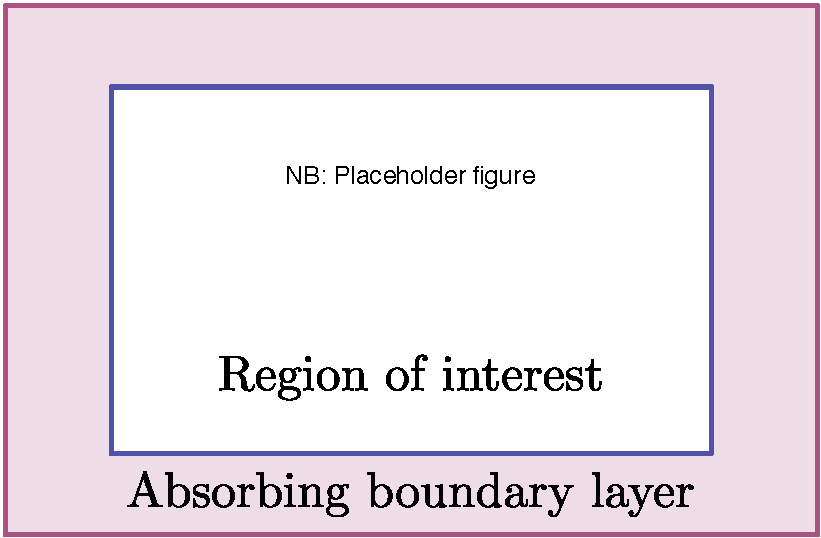
\includegraphics[width=8cm]{RegionOfInterest}
    \caption{\label{Peaks:RegionOfInterest} A snapshot of the total density from a GP simulation corresponding to the system under discussion in this chapter. It can be observed that the atom laser density is decaying within the absorbing boundary layer. The region of interest and absorbing boundary layer are marked. The region of interest is the entire computational domain except for the absorbing boundary layer. The absorbing boundary layer has a width of $\unit[5]{\micro m}$.}
\end{figure}

The rate and distribution with which momentum leaves the region of interest can be determined by considering the equation of motion for the wavenumber density in the region of interest,
\begin{align}
    \frac{\partial }{\partial t}\abs{\widetilde{\psi}_\text{roi}(\bm{k}, t)}^2 &= 2 \Re \left\{ \widetilde{\psi}_\text{roi}^*(\bm{k}, t) \frac{\partial }{\partial t}\widetilde{\psi}_\text{roi}(\bm{k}, t) \right \},
\end{align}
where $\widetilde{\psi}_\text{roi}(\bm{k}, t)$ is the Fourier transform of the restricted wavefunction $\psi_\text{roi}(\bm{x}, t)$, which is defined to be nonzero only within the region of interest. The equation of motion for $\widetilde{\psi}_\text{roi}(\bm{k}, t)$ is
\begin{align}
    \label{Peaks:PsikROIEquationOfMotion}
    \frac{\partial}{\partial t} \widetilde{\psi}_\text{roi}(\bm{k}, t) &= -\frac{i}{\hbar} \mathcal{F}\left[\left(-\frac{\hbar^2 \nabla^2}{2M} + V(\bm{x}) + U \abs{\psi_\text{roi}(\bm{x}, t)}^2\right) \psi_\text{roi}(\bm{x}, t)\right](\bm{k}),
\end{align}
where $\mathcal{F}[f(\bm{x})](\bm{k})$ denotes the Fourier transform of the function $f(\bm{x})$. While the potential and interaction terms in \eqref{Peaks:PsikROIEquationOfMotion} redistribute momentum, it is only due to the kinetic term that momentum will leave the region of interest. To see that this is true, consider a Hamiltonian with no kinetic term. In this case the local phase of the wavefunction will rotate, but the density distribution will remain unchanged. Hence it will be the kinetic term in \eqref{Peaks:PsikROIEquationOfMotion} that will determine the momentum density flux leaving the region of interest.

The Fourier transform of the kinetic term in \eqref{Peaks:PsikROIEquationOfMotion} can be evaluated to give the momentum density flux $\Phi(\bm{k}, t)$ leaving the region of interest in terms of a surface integral over the boundary of the region of interest,
\begin{align}
    \Phi(\bm{k}, t) & = -\frac{\partial }{\partial t}\abs{\widetilde{\psi}_\text{roi}(\bm{k}, t)}^2\bigg|_\text{kinetic}\\
    & = -2 \Re \left\{ \frac{i \hbar}{2 M} \widetilde{\psi}_\text{roi}^*(\bm{k}, t) \frac{1}{(2 \pi)^{\frac{3}{2}}}\oiint e^{-i \bm{k}\cdot \bm{x}} \Big[ \nabla \psi_\text{roi}(\bm{x}, t) + i \bm{k} \psi_\text{roi}(\bm{x}, t)\Big] \cdot d \bm{A} \right\}.
    \label{Peaks:MomentumDensityFluxSurfaceIntegral}
\end{align}
The $\psi_\text{roi}(\bm{x}, t)$ and $\nabla\psi_\text{roi}(\bm{x}, t)$ terms to be evaluated at the boundary in \eqref{Peaks:MomentumDensityFluxSurfaceIntegral} should be understood to be defined by the limit from the interior of the region of interest. While \eqref{Peaks:MomentumDensityFluxSurfaceIntegral} is the most direct way of evaluating $\Phi(\bm{k}, t)$, it is a computationally inefficient method as it requires the calculation of a surface integral for every point $\bm{k}$ at which we wish to evaluate $\Phi(\bm{k}, t)$. 

A more efficient method can be found by instead considering the evolution of the wavenumber density on the entire computational domain. The momentum flux density that left the region of interest enters the absorbing boundary layer through a term like \eqref{Peaks:MomentumDensityFluxSurfaceIntegral}, but leaves at a slightly later time due to the negative imaginary potential. As it is not the temporal dynamics of $\Phi(\bm{k}, t)$ in which we are interested, but just the distribution of momentum that left the region of interest at \emph{any} time, this delay is unimportant. On the entire computational domain, the two kinetic transport terms will cancel leaving the term due to the negative imaginary potential. Assuming that the mean-field interaction energy of the wavefunction reaching the absorbing boundary layer is small compared to its kinetic energy, the momentum flux density leaving the computational domain is given by
\begin{align}
    \label{Peaks:MomentumDensityFlux}
    \Phi(\bm{k}, t)&=\frac{2}{\hbar} \Re \left\{ \widetilde{\psi}^*(\bm{k}, t) \mathcal{F}'\left[ V_I(\bm{x}) \psi(\bm{x}, t)\right](\bm{k}) \right\},
\end{align}
where $\mathcal{F}'$ is the appropriate Fourier-like transform that connects the spatial and spectral representations of the wavefunction $\psi$, and guarantees the artificial boundary conditions are satisfied. Equation \eqref{Peaks:MomentumDensityFlux} is a more efficient method of evaluating $\Phi(\bm{k}, t)$ than \eqref{Peaks:MomentumDensityFluxSurfaceIntegral} as it only requires two Fourier-like transforms to evaluate $\Phi(\bm{k}, t)$ for all $\bm{k}$, instead of one surface integral \emph{for each} $\bm{k}$.

The information provided by either \eqref{Peaks:MomentumDensityFluxSurfaceIntegral} or \eqref{Peaks:MomentumDensityFlux} will only be as good as the absorbing boundary layer. While for a perfect absorbing boundary layer $\int \Phi(\bm{k}, t)\, dt$ would exactly equal the lost momentum density from the region of interest, for an imperfect absorbing boundary layer $\int \Phi(\bm{k}, t)\, dt$ will also include contributions due to any reflection from or transmission through the boundary layer. 

An example calculation of $\Phi(\bm{k}, t)$ for a finite absorbing boundary layer is given in \sectionref{MethodsAppendix:MomentumDensityFluxExampleCalculation}. There it is demonstrated that $\Phi(\bm{k}, t)$ is an accurate method for determining the rate of loss of momentum density from a region of space for the same range of momenta for which the absorbing boundary layer is itself accurate.

\parasep

The simulations described in the remainder of this chapter use the method presented in this section to determine the momentum distribution of atoms that have left computational domain. This momentum distribution is then propagated classically under gravity to find the corresponding density distribution on the MCP detector below the condensate. This classical propagation was performed by \emph{Mattias Johnsson}. Note that due to the use of cylindrical symmetry, the correct Fourier-like transform for use in \eqref{Peaks:MomentumDensityFlux} is the Hankel (or Bessel) transform \citep{ArfkeyWeber}.

% \subsection{Next section}
% Things that need to be discussed:
% \begin{enumerate}
%     \item The Theorist's on-resonance case. This is important because it shows agreement with the Floquet exponents calculated in an earlier section.
%     \item In this case, we need to perform both TW and GP simulations demonstrating that the peaks are only observed in the TW case and they obey the usual stuff. At this point we need to say why we are only using a two-level model here. If the Hankel simulations are working, then we will use those for these results and also try a three-level (proper) version.
%     \item Experimentalist's on-resonance case. Show the detuning plot so that we know exactly what the difference is and why. Extra points may need to be calculated for that curve. Then show the GP and TW results in the appropriate limit. Here is where we need to argue about how things are related to one another.
%     \item Future work and conclude.
% \end{enumerate}
% 
% Most of these sections can be written before the figures are available. The final figures can then be added as they are completed.

\subsection{Equations of motion}

Having described the calculational techniques that will be used, we will now turn to the description of the Gross-Pitaevskii and Truncated Wigner equations that were used to model the experiment. The GP equations that correspond to the master equation \eqref{Peaks:MasterEquation} are
\begin{subequations}
    \label{Peaks:3DGPEquations}
    \begin{align}
        \begin{split}
            i \hbar \frac{\partial }{\partial t}\Psi_1 &= \frac{-\hbar^2 \nabla^2}{2 M} \Psi_1 + \big(V_\text{trap}(\bm{x}) - i V_I(\bm{x})\big)\Psi_1 + \sqrt{2} \hbar \Omega \Psi_0 \\
            & \relphantom{=} + c_0 \sum_j \abs{\Psi_j}^2 \Psi_1 + c_2\left(\abs{\Psi_1}^2 + \abs{\Psi_0}^2 - \abs{\Psi_{-1}}^2 \right) \Psi_1 + c_2 \Psi_{-1}^*\Psi_0^2 \\
            & \relphantom{=} - i \hbar\frac{3}{2}K^\text{(unpol)}_{^{4}\text{He}} \left(2\abs{\Psi_{-1}}^2 \Psi_1 - \Psi_{-1}^* \Psi_0^2\right),
        \end{split}\\
        \begin{split}
            i \hbar \frac{\partial }{\partial t}\Psi_0 &= \frac{-\hbar^2 \nabla^2}{2 M} \Psi_0 + \big(\hbar \Delta - i V_I(\bm{x}) \big)\Psi_0 + \sqrt{2} \hbar \Omega \Psi_1 + \sqrt{2}\hbar\Omega \Psi_{-1} \\
            & \relphantom{=} + c_0 \sum_j \abs{\Psi_j}^2 \Psi_0 + c_2\left(\abs{\Psi_1}^2 + \abs{\Psi_{-1}}^2 \right) \Psi_0 + 2 c_2 \Psi_{0}^*\Psi_1\Psi_{-1} \\
            & \relphantom{=} - i \hbar\frac{3}{2}K^\text{(unpol)}_{^{4}\text{He}} \left(\abs{\Psi_{0}}^2 \Psi_0 - 2\Psi_{0}^* \Psi_1\Psi_{-1}\right),
        \end{split}\\
        \begin{split}
            i \hbar \frac{\partial }{\partial t}\Psi_{-1} &= \frac{-\hbar^2 \nabla^2}{2 M} \Psi_{-1} + \big(-V_\text{trap}(\bm{x}) + 2 \hbar \Delta - i V_I(\bm{x})\big)\Psi_{-1} + \sqrt{2} \hbar \Omega \Psi_0 \\
            & \relphantom{=} + c_0 \sum_j \abs{\Psi_j}^2 \Psi_{-1} + c_2\left(-\abs{\Psi_1}^2 + \abs{\Psi_0}^2 + \abs{\Psi_{-1}}^2 \right) \Psi_{-1} + c_2 \Psi_{1}^*\Psi_0^2 \\
            & \relphantom{=} - i \hbar\frac{3}{2}K^\text{(unpol)}_{^{4}\text{He}} \left(2\abs{\Psi_{1}}^2 \Psi_{-1} - \Psi_{1}^* \Psi_0^2\right),
        \end{split}
    \end{align}
\end{subequations}
where $\displaystyle V_\text{trap}(\bm{x}) = \frac{1}{2} M \left(\omega_r^2 r^2 + \omega_z^2 z^2 \right)$ is the trapping potential, $\hbar \Delta$ is the detuning in energy of the resonant outcoupling surface from the centre of the condensate, $c_0 = (g_0 + 2 g_2)/3$, $c_2 = (g_2 - g_0)/3$, where $g_S = 4 \pi \hbar^2 a_S/M$ is the nonlinear interaction strength, and $a_S$ is the $s$-wave scattering length for the total hyperfine spin $S$ channel (refer to \sectionref{BackgroundTheory:Helium}). A derivation of the Penning ionisation terms in \eqref{Peaks:3DGPEquations} is given in \sectionref{PenningIonisationAppendix:GP}.

The Truncated Wigner equations corresponding to the master equation \eqref{Peaks:MasterEquation} are very similar to \eqref{Peaks:3DGPEquations} but with the addition of noise-correction terms. In Stratonovich form, the equations of motion for the stochastic wavefunctions are approximately
% See MolecularScattering.nb for the derivation of the Penning ionisation terms
\begin{align}
    \label{Peaks:3DTWEquations}
    \begin{split}
        \left. i \hbar \,d\bm{\Psi}\right|_\text{TW} &\approx \left. i \hbar \frac{\partial }{\partial t}\bm{\Psi}\right|_\text{GP} dt - \left(2 c_0 + c_2 \right)\frac{1}{\Delta V}\bm{\Psi}\, dt\\
        &\relphantom{\approx} + i\sqrt{ \hbar V_I(\bm{x})} \,d\bm{W}(\bm{x}) + i \hbar\sqrt{3 \Kunpol}
        \begin{pmatrix}
            \Psi_{-1}^*\\
            \Psi_0^*\\
            \Psi_1^*
        \end{pmatrix} dW_p(\bm{x}),
    \end{split}
\end{align}
where $\Delta V$ is the computational grid's volume element (for irregularly spaced grids such as those that used for cylindrically symmetric problems, $\Delta V$ is the local Gaussian quadrature weight \citep{Ronen:2006}), $\bm{\Psi} = \left(\Psi_1, \Psi_0, \Psi_{-1} \right)^T$ and $d \bm{W}(\bm{x}) = \big(dW_1(\bm{x}), dW_0(\bm{x}), dW_{-1}(\bm{x})\big)^T$ and $dW_p(\bm{x})$ are the complex Gaussian noises satisfying
\begin{align}
    \overline{dW_i(\bm{x})\, dW_j(\bm{x}')} &= 0 \\
    \overline{dW_i(\bm{x})\, dW_j^*(\bm{x}')} &= \frac{1}{\Delta V}\delta_{ij}\delta_{\bm{x},\bm{x}'}\,dt, \label{Peaks:ComplexNoiseExpectationValue}
\end{align}
where $\overline{(\cdot)}$ denotes the expectation value taken with respect to the noises. The usual spatial Dirac delta function in \eqref{Peaks:ComplexNoiseExpectationValue} has been replaced by a Kronecker delta function scaled by the inverse volume element due to the discrete nature of the computational grid.

The additional terms given by \eqref{Peaks:3DTWEquations} can be interpreted in the following way, the $\Delta V^{-1}$ term corrects for the additional `virtual' particles added to the initial state of the stochastic wavefunctions (refer to \sectionref{BackgroundTheory:TruncatedWigner}), the $d \bm{W}$ term corrects for the loss of virtual particles due to the absorbing boundary layer and the $dW_p$ term does similarly for virtual particles lost due to Penning ionisation.

The approximation made in obtaining \eqref{Peaks:3DTWEquations} was to neglect $\Delta V^{-1}$ compared to the field occupations $\abs{\Psi_1}^2$, $\abs{\Psi_0}^2$, $\abs{\Psi_{-1}}^2$ in the Penning ionisation noise term. This is justified for large occupations where Penning ionisation will be significant. The approximation cannot be made where the density is low, but at these locations the Penning ionisation process itself can be neglected as the associated rate constant will have decreased proportionally with the density. A derivation of the Penning ionisation noise term in \eqref{Peaks:3DTWEquations} is given in \sectionref{PenningIonisationAppendix:TW}.

In an ideal world, our job would be done once a set of equations has been derived that can model a system. Unfortunately, technical considerations often limit which problems are and are not feasible to solve. In this case, although the GP equations given in \eqref{Peaks:3DGPEquations} can be solved in a couple of days on a supercomputer, \eqref{Peaks:3DTWEquations} represents a much more challenging problem. Not only do these equations need to be solved a large number of times ($N_\text{paths} \gtrsim 100$) for different initial conditions, but algorithms for solving stochastic differential equations are limited to a lower order\footnote{For example, Runge-Kutta type algorithms are limited to a one-step error of $\displaystyle O(\Delta t^\frac{3}{2})$ \citep{Ruemelin:1982}. Algorithms using higher-order moments of the noises are able to achieve a global error of $\displaystyle O(\Delta t)$ \citep{Burrage:2004}.} than those that can be used for deterministic differential equations hence  significantly smaller time steps are required for solving stochastic differential equations. This problem is mainly due to the $\Psi_{-1}$ state which, due to the antitrapping potential, has a kinetic energy $\sim 40$ times larger than the $\Psi_{0}$ atoms at the edge of the computational domain $\unit[60]{\micro m}$ away from the centre of the condensate in the radial direction. The computational domain cannot be restricted to be tighter due to the requirement that the mean-field energy of the $\Psi_{0}$ atoms be negligible compared to their kinetic energy for the absorbing boundary layer to be effective. While it is for these practical reasons that we must neglect the $\Psi_{-1}$ state, we are physically justified in doing so by the same arguments given at the start of \sectionref{Peaks:PerturbativeApproach}.

In the next sections the behaviour of the atom laser in the cases of outcoupling from the centre of the condensate (resonant outcoupling) and outcoupling from a detuned surface where the atom laser flux is maximised are considered.

\subsection{Resonant outcoupling}

As a verification of the results of \sectionref{Peaks:PerturbativeApproach} we first consider outcoupling from the centre of the condensate ($\Delta = 0$). This is the case that corresponds most closely with that of the homogenous condensate considered in \sectionref{Peaks:PerturbativeApproach} because the shape of the outcoupling surfaces (see \figureref{Peaks:OutcouplingSurfaces}) restricts outcoupling to the centre of the condensate where the density is a local maximum; here the condensate is locally homogeneous.

\begin{figure}
    \centering
    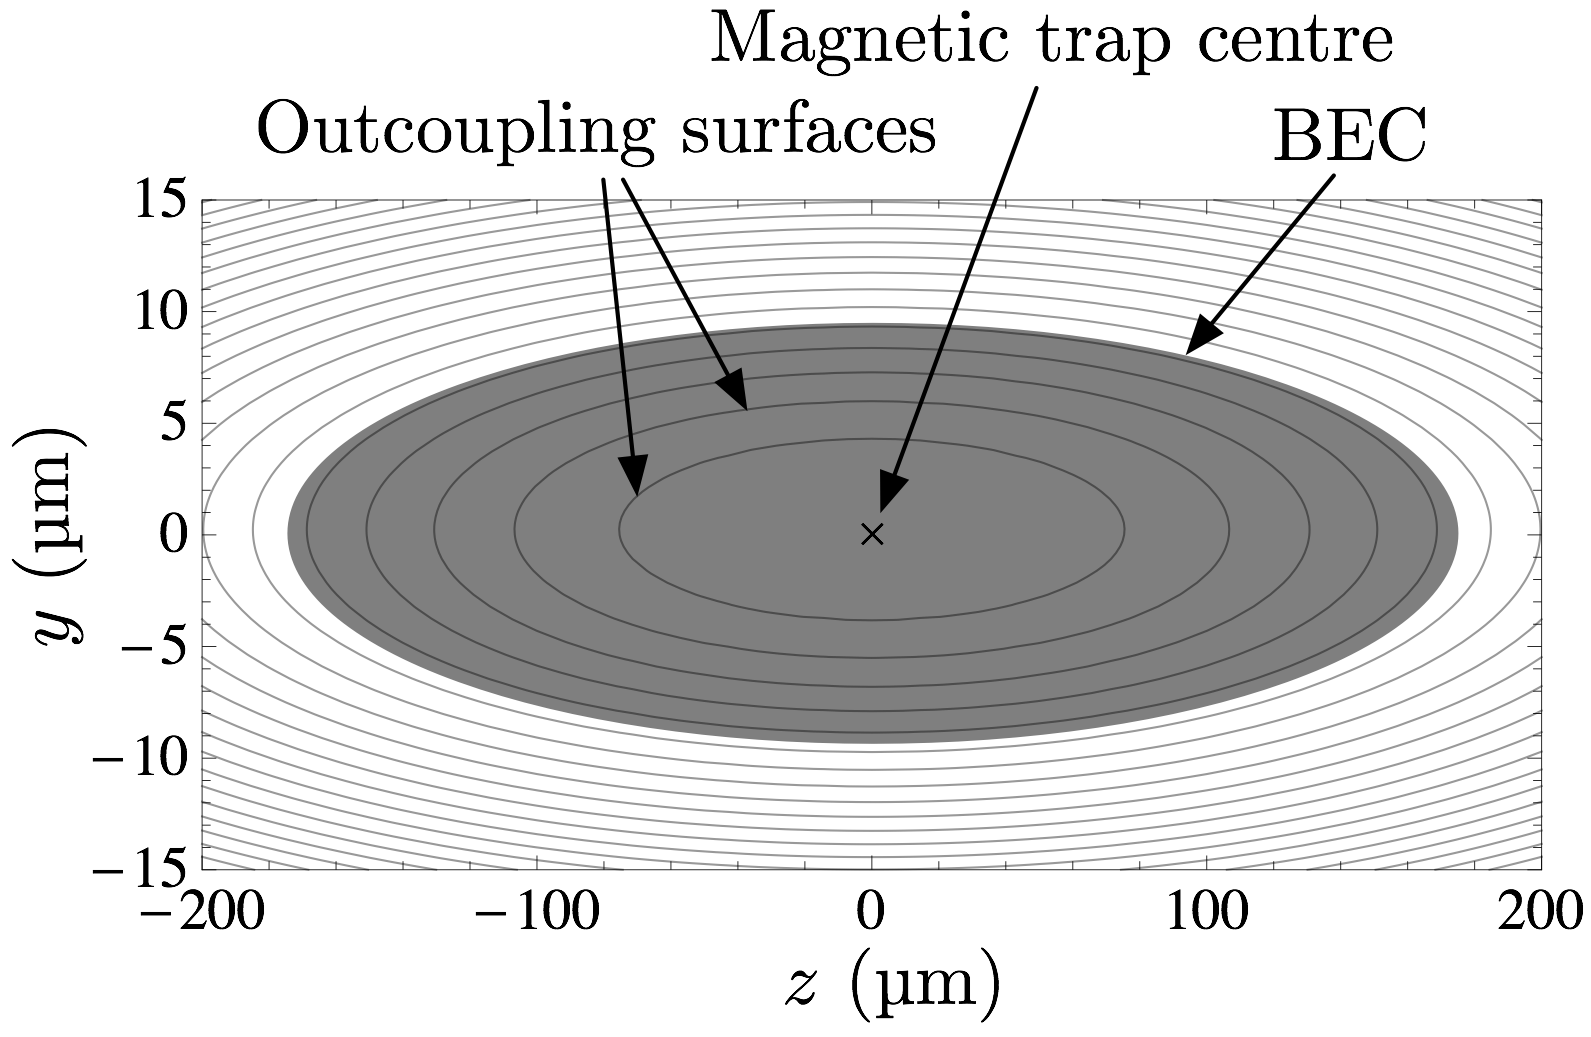
\includegraphics[width=8cm]{OutcouplingSurfaces}
    \caption{\label{Peaks:OutcouplingSurfaces} Outcoupling surfaces of the He* condensate under consideration in this chapter. The small gravitational sag of $y_\text{sag} = \unit[0.2]{\micro m}$ means that the centre of the trap and the centre of the condensate almost exactly coincide. Hence the outcoupling surfaces are approximately centred on the centre of the condensate. The contours pictured are equally-spaced in energy.}
\end{figure}

The results of the GP and TW simulations for the case of resonant outcoupling are presented in \figureref{Peaks:TheoryZeroDetuningResults}. As expected, the spontaneously-seeded dynamical instabilities predicted in \sectionref{Peaks:PerturbativeApproach} are not observed in the GP simulations where spontaneous scattering does not occur. Moreover, two of the dynamical instabilities predicted in \sectionref{Peaks:PerturbativeApproach} are observed in the results of the TW simulation with the third indistinguishable from the vacuum fluctuations due to the small number of paths used. Although Penning ionisation was not considered in \sectionref{Peaks:PerturbativeApproach}, it can be seen from the results presented in \figureref{Peaks:TheoryZeroDetuningResults} that the instabilities have not been suppressed by Penning ionisation.

As the instabilities in \figureref{Peaks:TheoryZeroDetuningResults}(e) are outcoupled it can be observed that they accelerate along the radial direction forming momentum cones such as those pictured in \figureref{Peaks:Schematic}. When these momentum cones fall onto the detector they are vertically integrated to produce the well-defined peak-like structures in \figureref{Peaks:TheoryZeroDetuningResults}(f). Although these instabilities are entangled upon formation, it is unlikely that any useful entanglement will survive the outcoupling process as it is only the $\Psi_0$ and $\Psi_{-1}$ states that can escape the condensate. Despite this, it is likely that there will be number-difference squeezing between opposite points on the momentum cones as the characteristic time for the outcoupling process $\sim \unit[3]{ms}$ is much less than the time for an atom to undergo an oscillation in the weak trapping direction of $\sim \unit[18]{ms}$. Consequently, it is unlikely that the $\Psi_1$ component of the instability will remain in the condensate long enough for its momentum in the weak trapping dimension to change significantly. This number-difference squeezing between opposite points on the momentum-cones would be observed as a number difference squeezing between the structures on the opposite sides of the main atom laser profile in \figureref{Peaks:TheoryZeroDetuningResults}(f). Unfortunately, due to the computational difficulty of the problem, it is not at present possible to theoretically verify the claim of number-difference squeezing due to the large number of paths that would be required for any results to have statistical significance.

\begin{figure}
    \centering
    FIXME: Perform final simulations and create figure.
    \caption{\label{Peaks:TheoryZeroDetuningResults} Simulation results for outcoupling from the centre of the condensate. Left figures (a), (c) and (e) plot the momentum density of the untrapped state at $t=\unit[\text{FIXME}]{ms}$. Right figures (b), (d) and (f) plot the density profiles that would be observed on the MCP detector. The upper figures (a) and (b) plot the results of a GP model including all $m_F$ atomic levels. Middle figures (c) and (d) plot the results of a reduced GP model where the $m_F=-1$ is assumed negligible, lower figures (e) and (f) correspond to a Truncated Wigner simulation for the same system with $N_\text{paths} = \text{FIXME}$. The wavenumbers predicted to be unstable by the perturbation analysis performed in \sectionref{Peaks:PerturbativeApproach} are marked in (e).}
\end{figure}

\subsection{Maximum atom laser flux}

In the previous section the behaviour of the atom laser in the case of outcoupling from the centre of the condensate was considered. While in this case it is comparatively easy to understand the dynamics as the condensate is locally homogeneous, the general case of detuned outcoupling is significantly more difficult to understand due to the inherent multimode behaviour. Naturally\footnote{FIXME: I can't get away with saying this.}, the experimental results shown in \figureref{Peaks:ExperimentalResults} were for the case of a detuning of $\Delta = 2\pi \times \unit[6.5]{kHz}$ which is a significant fraction of the chemical potential $\mu = 2\pi \times \unit[18]{kHz}$. The reason for this detuning is that the atom laser flux is very small when outcoupling from the centre of the condensate making detection difficult. In a simple model, the outcoupled atom laser flux is proportional to the surface area of the outcoupling surface times the average density over that surface. Outcoupling from the centre of the condensate will therefore lead to a small atom laser flux. Detuning will cause this atom laser flux to increase as the surface area increases before decreasing again as the condensate density drops off towards the edge of the condensate. This behaviour is plotted in \figureref{Peaks:DetuningCurve}. The experimental results presented in \figureref{Peaks:ExperimentalResults} were for the detuning which maximises the atom laser flux, which can be seen from \figureref{Peaks:DetuningCurve} to be $\Delta = 2\pi \times \unit[6.5]{kHz}$.

\begin{figure}
    \centering
    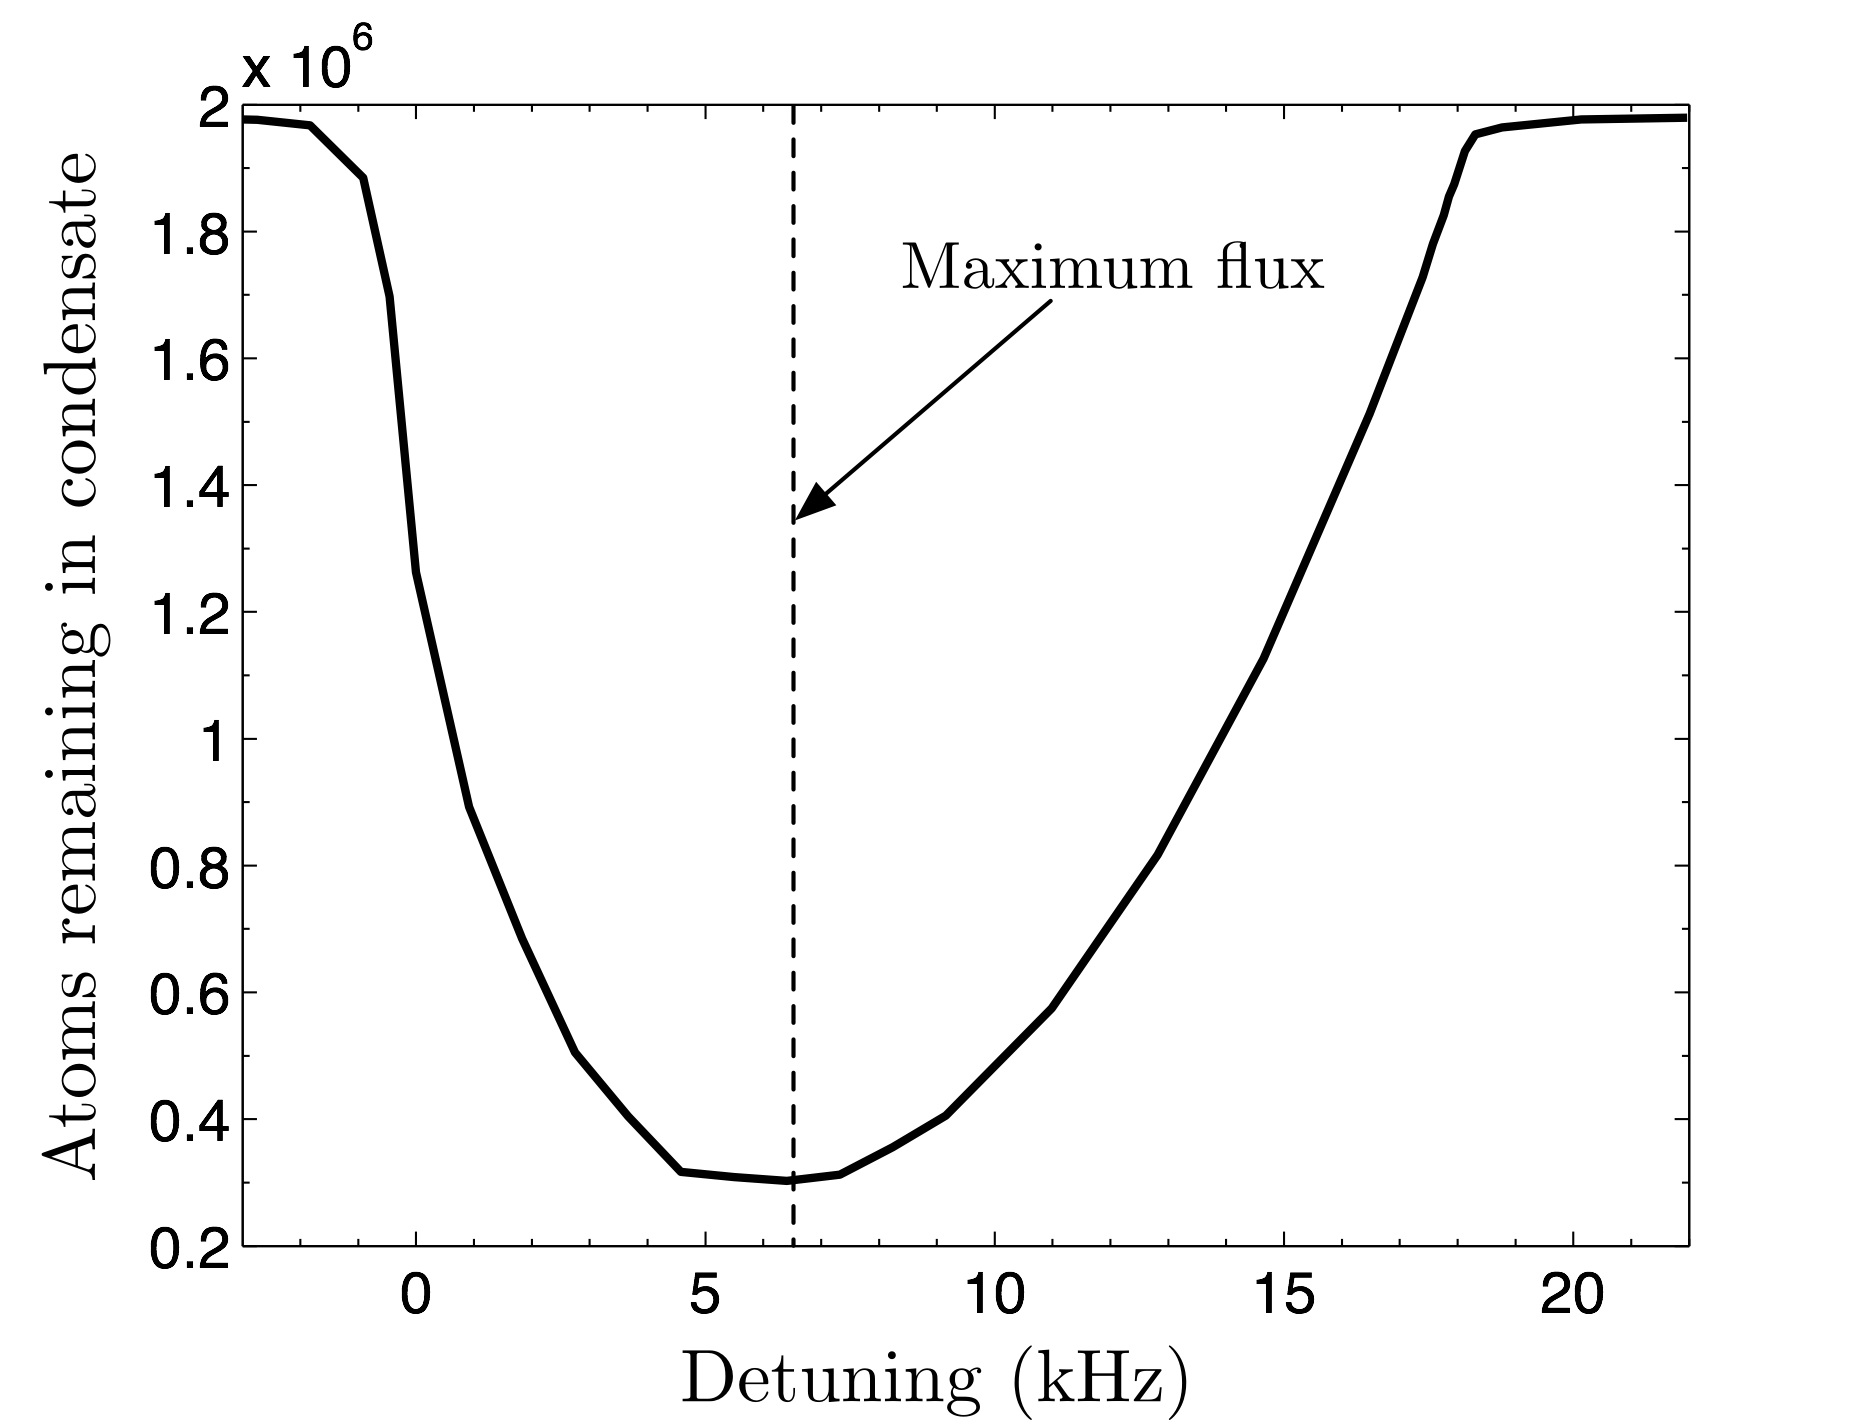
\includegraphics[width=8cm]{DetuningCurve}
    \caption{\label{Peaks:DetuningCurve} Theoretical calculation of the number of atoms remaining in the condensate after $\unit[10]{ms}$ of outcoupling at a Rabi frequency of $\Omega = \unit[210]{Hz}$ as a function of the detuning of the rf outcoupling from the centre of the condensate. The results shown are obtained from simulations of the 3D GP equations for the condensate under consideration.}
\end{figure}

The results for GP and TW simulations of the experiment with a detuning of $\Delta = 2\pi \times \unit[6.5]{kHz}$ are shown in \figureref{Peaks:TheoryMaxFluxDetuningResults}. A discussion is needed here.

\begin{figure}
    \centering
    FIXME: Perform final simulations and create figure.
    \caption{\label{Peaks:TheoryMaxFluxDetuningResults} Simulation results for outcoupling with a detuning of $\Delta = 2\pi \times \unit[6.5]{kHz}$ from the centre of the condensate. Left figures (a), (c) and (e) plot the momentum density of the untrapped state at $t=\unit[\text{FIXME}]{ms}$. Right figures (b), (d) and (f) plot the density profiles that would be observed on the MCP detector. The upper figures (a) and (b) plot the results of a GP model including all $m_F$ atomic levels. Middle figures (c) and (d) plot the results of a reduced GP model where the $m_F=-1$ is assumed negligible, lower figures (e) and (f) correspond to a Truncated Wigner simulation for the same system with $N_\text{paths} = \text{FIXME}$.}
\end{figure}


\subsection{Entangled beams?}
Discuss the prospect of entangled beams, work down to correlated beams. Specifically, number-difference correlations. Can't be shown to be true or false given the current results. Limited by stuff, but ultimately, not that interesting. A basic comparison to the colliding-condensates experiments. Squeezing has been proposed in similar kinds of systems. Such experiments must take care to avoid the instabilities discussed in the earlier section.

\section{Summary}

\hrule






We need to discuss the artificial boundary conditions used. Mention that Fourier boundary conditions were used in the paper, which are less than optimal, but used due to the limitations of the tools at hand. That said, the results presented here use the Hankel transform (discussed in a numerical methods appendix) and differ negligibly (they bloody well better) from the results in the paper.

We also need to discuss the method used to obtain the momentum flux density.

\hrule



As noted in the previous section, a GP equation model corresponding to \eqref{Peaks:MasterEquation} will be unable to reproduce the instability as it is spontaneously-seeded. 


% 
% Two options: 
% * Describe the Hamiltonian used in the paper, and risk it being noticed.
%     - Under review, this may be noticed, and if that occurs, it would lead to very, very bad things.
% * Use the other Hamiltonian and justify neglecting the mF=-1 state.
%     - The approximation will be noticed, and discussed. The question may be asked why I didn't try and not make this approximation.
% 
% The direction of the previous section has been in the line of the two-level model. But it leaves it so open to questions being asked.
% Alternatively, I can solve *different* models for different reasons. I would then need to justify only using a two-level model for TW simulations, but can get away with a full 3D model for GP simulations. This appears to be the best approach.
% 
% Must justify using only two levels for TW, but three for GP.
% This requires doing the TW and GP simulations again but using Hankel transforms.
% 
% Method: 
%     2-level TW to see what the instabilities give rise to.
%     2-level TW at correct detuning to see what happens.
%     3-level GP at correct detuning for final results.
% This method requires a justification of 2-level for TW. A 2-level model can be justified in terms of checking what the previous analysis gives rise to, and then a full 3-level model could be discussed. In fact, we could discuss early on that the detuning doesn't correspond to the centre of the condensate (probably reference an earlier chapter), do a 2-level TW corresponding to that to see what happens, and then do 3-level TW and GP corresponding to the actual outcoupling position used in the experiment. That would then require justification of the link between the two phenomena. It's physics, it has to work. This justification must stand up to scrutiny by Craig and John. Oooh. I could even admit that the link isn't entirely solid. I could argue that the complicated dynamics would prevent any analytic determination of the behaviour, it could be the subject of future work to see if these bloody things are correlated.
% 
% This then requires some motivation that the two phenomena are related. Something about the sweeping resonance crap I used before. One really good way of doing this would be by analogy. Some analogy with some other crap that is also produced in a similar way. The other possibility would be the initial outcoupling process leading to a resonance sweep. Initial dynamics. That must be it. Fourier arguments. I then need a density-dependent resonance. Three-levels. Complicated stuff. Wave hands.
% 
% I can justify the 2-level. No I can't. It's bloody deterministic... Unless I include the proper noise due to the absorbing boundary and/or penning ionisation. Oooh. That could actually save my bacon.
% 
% And it would actually be true. Neglect the Penning ionisation noise terms. Somewhere I must discuss the correct Master equation term for Penning ionisation. I'm guessing that's going to need to be in an earlier chapter that discusses the properties of Rubidium and Helium. And I should somewhere mention Lesa's work on building a dual-species Rubidium-Helium BEC.
% 
% Semi-Implicit low-order algorithms to the rescue... Whether I actually calculate it that way or not... we'll see.
% 
% Can I say things that went wrong? Things to avoid?
% 
% I can even perform 2-level and 3-level GP simulations of the zero-detuning case. I just can't do a 3-level TW simulation there.
% 
% So: start with the full master equation and work down from there as we go. The remaining question is how best to write that master equation.
% 
% 
% 
% 
% 
% 
% \begin{align}
%     K_{^{4}\text{He}}
% \end{align}
% 
% a multimode calculation of the entire BEC was performed, which is discussed in this section.
% 
% 
% The Hamiltonian for the system that 
% 
% As the instabilities discussed in the previous section were seeded by vacuum fluctuations, it will be expected that 
% 
% For the same reasons mentioned at the start of \sectionref{Peaks:PerturbativeApproach}, the $m_F=-1$ state can be neglected. This approximation is only necessary for technical reasons, as the full 3D calculation requires excessive computational resources. The Hamiltonian under consideration is then the same as \eqref{Peaks:InitialHamiltonian} but with the addition of the state-dependent potentials $V_i(\bm{x})$,
% \begin{align}
%     \begin{split}
%     \hat{H} &= \sum_i \int d\bm{x}\, \hat{\Psi}_i^\dagger \left(\frac{-\hbar^2 \nabla^2}{2 M} + V_i(\bm{x})- \mu\right)\hat{\Psi}_i^{\phantom{\dagger}} + \frac{1}{2} \sum_{i j} U_{i j}\int d\bm{x}\, \hat{\Psi}_i^\dagger \hat{\Psi}_j^\dagger \hat{\Psi}_j^{\phantom{\dagger}} \hat{\Psi}_i^{\phantom{\dagger}}\\
%             &\phantom{=} + \hbar \Omega \int d\bm{x}\, \left(\hat{\Psi}_1^\dagger \hat{\Psi}_0^{\phantom{\dagger}} + \hat{\Psi}_0^\dagger \hat{\Psi}_1^{\phantom{\dagger}}\right).
%     \end{split}
% \end{align}

